\part{SNIPPETS}

\chapter{Snippet [COUNT policy]}

\begin{wrapfigure}{r}{0pt}
\resizebox{0.4\textwidth}{!}{

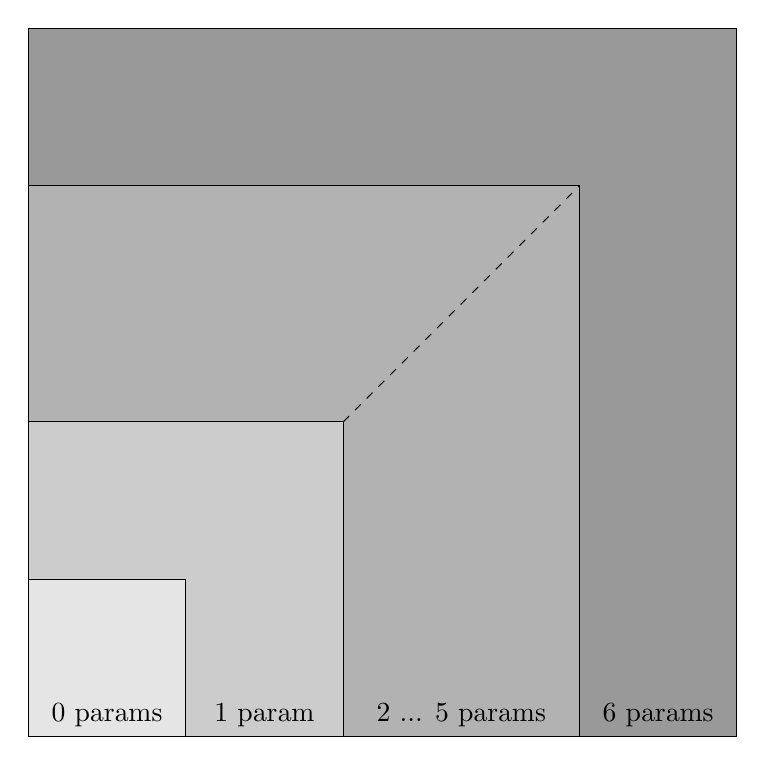
\begin{tikzpicture}


\fill[black!40!white] (0,0) rectangle (9,9);
\fill[black!30!white] (0,0) rectangle (7,7);
\fill[black!20!white] (0,0) rectangle (4,4);
\fill[black!10!white] (0,0) rectangle (2,2);


\draw (0,0) --node[anchor=south] {0 params} (2,0)  -- (2,2) -- (0,2) -- (0,0) ;

\draw (0,0) -- (2,0) --node[anchor=south] {1 param} (4,0) -- (4,4) -- (0,4) -- (0,0);


\draw (0,0) --(4,0) --node[anchor=south] {2 ... 5 params} (7,0) -- (7,7) -- (0,7) -- (0,0);

\draw (0,0) --(7,0) --node[anchor=south] {6 params} (9,0) -- (9,9) -- (0,9) -- (0,0);

\draw[dashed] (4,4) -- (7,7);
	
\end{tikzpicture}

}
\caption{COUNT policy schema}
\label{fig:COUNTschema}
\end{wrapfigure}

What we call the COUNT policy is essentially the policy introduced by typearmor\cite{typearmor}. The basic idea revolves aroung classifying calltargets by the number of parameters they provide and callsites by the number of paramters they require. Furthermore, generating 100\% precise measurements for such classification with binaries as the only source of information is rather difficult. Therefore overestimations of parameter count for callsites and underestimations of the parameter count for calltargets is deemed acceptable. This classification is based on the general purpose registers that the SystemV ABI designates as parameter registers and completely ignores other registers like floating point ones. The core of the COUNT policy is now to allow any callsite $cs$, which provides $c_{cs}$ parameters, to call any calltarget $ct$, which requires $c_{ct}$ parameters, iff $c_{ct} \leq c_{cs}$ holds. The main problem however, is that while their is a significant restriction of calltargets for the lower callsites, the restriction capability drops rather rapidly when reaching higher parameter counts, with callsites that use 6 or more parameters being able to call all possible calltargets:
\[
	\forall cs_1, cs_2.  c_{cs_1} \leq c_{cs_2} \Longrightarrow  \| \{ct \in \mathcal{F} | c_{ct} \leq c_{cs_1} \} \| \leq \| \{ct \in \mathcal{F} | c_{ct} \leq c_{cs_2}  \} \|
\]
One possible remedy would be the ability to introduce an upper bound for the classification deviation of parameter counts, however as of now, this does not seem feasible with current technology. Another possibility would be the overall reduction of callsites, which can access the same set of calltargets, a route we will explore within this work.

To aquire the classification of calltargets, a forward liveness analysis is used, which works rather well with 0 overestimations in 6 of 8 testargets and 1 overestimation in mysqld and postgres and perfect classification percentage between 67\% and 88\%. 
However the reaching analysis, which is used to classify callsites is more problematic with only 0 targets showing zero underestimations and all others ranging between 5\% and 17\%.


\chapter{Snippet [TYPE policy]}

\begin{figure}
\resizebox{\textwidth}{!}{
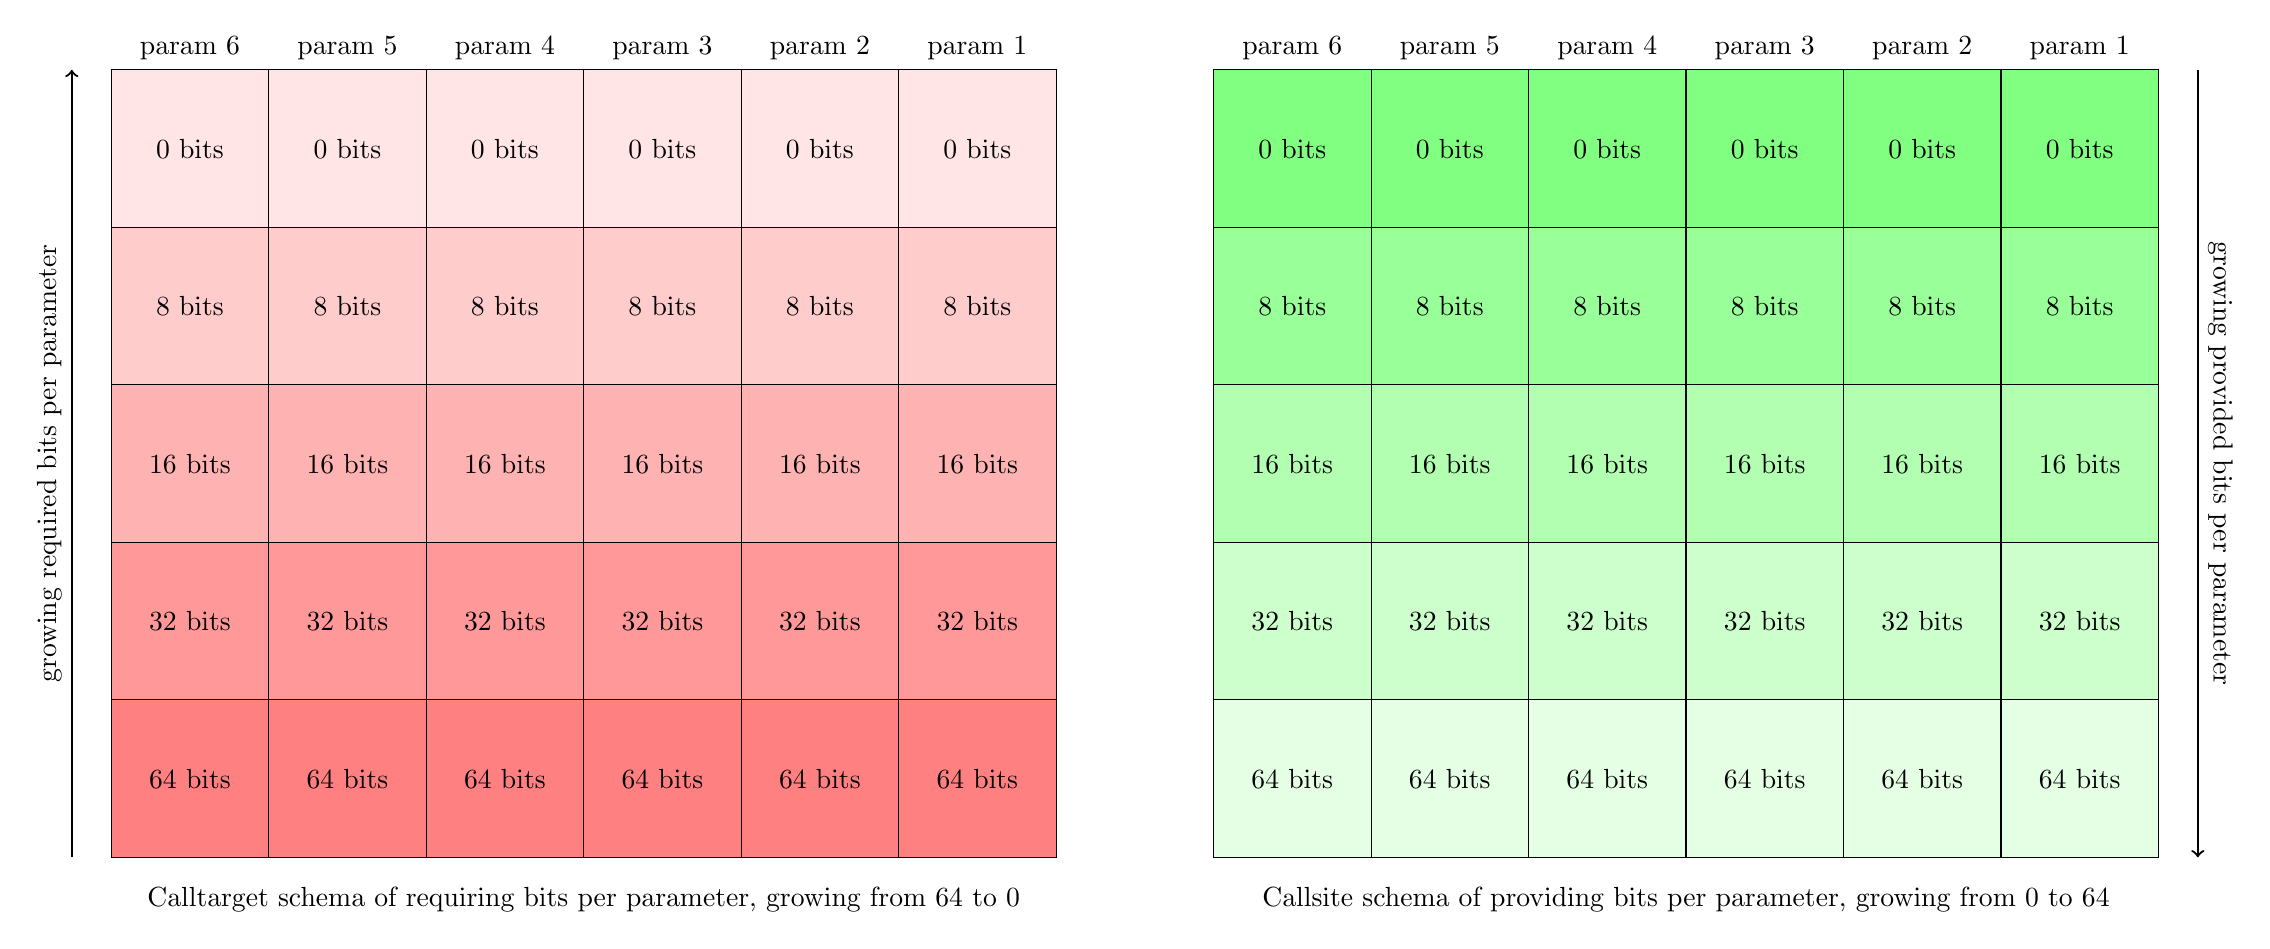
\begin{tikzpicture}

\fill[red!10!white] (0,10) rectangle (12,8);
\fill[red!20!white] (0,8) rectangle (12,6);
\fill[red!30!white] (0,6) rectangle (12,4);
\fill[red!40!white] (0,4) rectangle (12,2);
\fill[red!50!white] (0,2) rectangle (12,0);

\draw[thick,->] (-0.5,0) -- node[sloped, anchor=center, above] {growing required bits per parameter} (-0.5,10);
\draw[thick,->] (26.5,10) -- node[sloped, anchor=center, above] {growing provided bits per parameter} (26.5,0);

\draw[white](14,-0.25) -- node[anchor = north, black, thick] {Callsite schema of providing bits per parameter, growing from 0 to 64} (26,-0.25);
\draw[white](0,-0.25) -- node[anchor = north, black, thick] {Calltarget schema of requiring bits per parameter, growing from 64 to 0} (12,-0.25);

\draw (0,10) --node[anchor=south] {param 6} (2,10);
\draw (2,10) --node[anchor=south] {param 5} (4,10);
\draw (4,10) --node[anchor=south] {param 4} (6,10);
\draw (6,10) --node[anchor=south] {param 3} (8,10);
\draw (8,10) --node[anchor=south] {param 2} (10,10);
\draw (10,10) --node[anchor=south] {param 1} (12,10);

\draw (0,10) rectangle node[anchor=center] {0 bits} (2,8);
\draw (2,10) rectangle node[anchor=center] {0 bits} (4,8);
\draw (4,10) rectangle node[anchor=center] {0 bits} (6,8);
\draw (6,10) rectangle node[anchor=center] {0 bits} (8,8);
\draw (8,10) rectangle node[anchor=center] {0 bits} (10,8);
\draw (10,10) rectangle node[anchor=center] {0 bits} (12,8);

\draw (0,8) rectangle node[anchor=center] {8 bits} (2,6);
\draw (2,8) rectangle node[anchor=center] {8 bits} (4,6);
\draw (4,8) rectangle node[anchor=center] {8 bits} (6,6);
\draw (6,8) rectangle node[anchor=center] {8 bits} (8,6);
\draw (8,8) rectangle node[anchor=center] {8 bits} (10,6);
\draw (10,8) rectangle node[anchor=center] {8 bits} (12,6);

\draw (0,6) rectangle node[anchor=center] {16 bits} (2,4);
\draw (2,6) rectangle node[anchor=center] {16 bits} (4,4);
\draw (4,6) rectangle node[anchor=center] {16 bits} (6,4);
\draw (6,6) rectangle node[anchor=center] {16 bits} (8,4);
\draw (8,6) rectangle node[anchor=center] {16 bits} (10,4);
\draw (10,6) rectangle node[anchor=center] {16 bits} (12,4);

\draw (0,4) rectangle node[anchor=center] {32 bits} (2,2);
\draw (2,4) rectangle node[anchor=center] {32 bits} (4,2);
\draw (4,4) rectangle node[anchor=center] {32 bits} (6,2);
\draw (6,4) rectangle node[anchor=center] {32 bits} (8,2);
\draw (8,4) rectangle node[anchor=center] {32 bits} (10,2);
\draw (10,4) rectangle node[anchor=center] {32 bits} (12,2);

\draw (0,2) rectangle node[anchor=center] {64 bits} (2,0);
\draw (2,2) rectangle node[anchor=center] {64 bits} (4,0);
\draw (4,2) rectangle node[anchor=center] {64 bits} (6,0);
\draw (6,2) rectangle node[anchor=center] {64 bits} (8,0);
\draw (8,2) rectangle node[anchor=center] {64 bits} (10,0);
\draw (10,2) rectangle node[anchor=center] {64 bits} (12,0);

\fill[green!50!white] (14,10) rectangle (26,8);
\fill[green!40!white] (14,8) rectangle (26,6);
\fill[green!30!white] (14,6) rectangle (26,4);
\fill[green!20!white] (14,4) rectangle (26,2);
\fill[green!10!white] (14,2) rectangle (26,0);

\draw (14,10) --node[anchor=south] {param 6} (16,10);
\draw (16,10) --node[anchor=south] {param 5} (18,10);
\draw (18,10) --node[anchor=south] {param 4} (20,10);
\draw (20,10) --node[anchor=south] {param 3} (22,10);
\draw (22,10) --node[anchor=south] {param 2} (24,10);
\draw (24,10) --node[anchor=south] {param 1} (26,10);

\draw (14,10) rectangle node[anchor=center] {0 bits} (16,8);
\draw (16,10) rectangle node[anchor=center] {0 bits} (18,8);
\draw (18,10) rectangle node[anchor=center] {0 bits} (20,8);
\draw (20,10) rectangle node[anchor=center] {0 bits} (22,8);
\draw (22,10) rectangle node[anchor=center] {0 bits} (24,8);
\draw (24,10) rectangle node[anchor=center] {0 bits} (26,8);

\draw (14,8) rectangle node[anchor=center] {8 bits} (16,6);
\draw (16,8) rectangle node[anchor=center] {8 bits} (18,6);
\draw (18,8) rectangle node[anchor=center] {8 bits} (20,6);
\draw (20,8) rectangle node[anchor=center] {8 bits} (22,6);
\draw (22,8) rectangle node[anchor=center] {8 bits} (24,6);
\draw (24,8) rectangle node[anchor=center] {8 bits} (26,6);

\draw (14,6) rectangle node[anchor=center] {16 bits} (16,4);
\draw (16,6) rectangle node[anchor=center] {16 bits} (18,4);
\draw (18,6) rectangle node[anchor=center] {16 bits} (20,4);
\draw (20,6) rectangle node[anchor=center] {16 bits} (22,4);
\draw (22,6) rectangle node[anchor=center] {16 bits} (24,4);
\draw (24,6) rectangle node[anchor=center] {16 bits} (26,4);

\draw (14,4) rectangle node[anchor=center] {32 bits} (16,2);
\draw (16,4) rectangle node[anchor=center] {32 bits} (18,2);
\draw (18,4) rectangle node[anchor=center] {32 bits} (20,2);
\draw (20,4) rectangle node[anchor=center] {32 bits} (22,2);
\draw (22,4) rectangle node[anchor=center] {32 bits} (24,2);
\draw (24,4) rectangle node[anchor=center] {32 bits} (26,2);

\draw (14,2) rectangle node[anchor=center] {64 bits} (16,0);
\draw (16,2) rectangle node[anchor=center] {64 bits} (18,0);
\draw (18,2) rectangle node[anchor=center] {64 bits} (20,0);
\draw (20,2) rectangle node[anchor=center] {64 bits} (22,0);
\draw (22,2) rectangle node[anchor=center] {64 bits} (24,0);
\draw (24,2) rectangle node[anchor=center] {64 bits} (26,0);
\end{tikzpicture}
}

\caption{TYPE policy schema for callsites and calltargets}
\label{fig:TYPEschema}
\end{figure}
What we call the TYPE policy is the idea of not only relying on the parameter count but also on the type of a parameter. However due to complexity reasons, we are restricting ourselves to the general purpose registers, which the SystemV ABI designates as parameter registers. In general, these 64bit registers can be accessed in 4 different ways, one can access the whole 64bit register, the lower 32bit part, the lower 16bit part, or the lower 8bit part. Four general purpose registers can also directly access the higher 8bit part of the 16bit lower part, but for our purpose we also registers those as a 16bit access. Based on this information, we can assign a register one of 5 possible simplistic types $\mathcal{T} = {64, 32, 16, 8, 0}$. We also included the type 0 to model the absence of data within a register. Now similar to typearmor we also allow overestimation of types in callsites and underestimation of types in calltargets. However the matching idea is different, because as can we depict in Figure \ref{fig:TYPEschema}, the type of a calltarget and a callsite no longer depends solely on its parameter count, each callsite and calltarget has its type from the set of $\mathcal{T}^6$, with the following comparison operator:
\[
	u \leq_{type} v :\Longleftrightarrow  \forall_{i = 0}^{5} {u_i \leq v_i} , \text {with } u, v \in \mathcal{T}^6
\]
Again we allow any callsite $cs$ call any calltarget $ct$, when it fulfillst the requirement $ct \leq cs$. The way we represent this is by letting the type for a calltarget parameter progress from 64bit to 0bit - If a calltarget requires a 32bit value in its 1st parameter, it also should accept a 64bit value from its callsite - and similarly we let the type for a callsite progress from 0bit to 64bit - If a callsite provides a 32bit value in its 1st parameter it also provides a 16bit, 8bit and 0bit to a calltarget. Now the advantage of the TYPE policy in comparison to the COUNT policy is that while our type comparison implies the count comparison, the other direction does not hold. Meaning, just the having an equal or lesser number of parameters than a callsite, does no longer allow a calltarget being called there, thus restricting the number of calltargets per callsite even further. A function that requires 64bit in its first parameter, and 0bit in all other parameters, would have been callable by a callsite providing 8bit in its first and second parameter when using the COUNT policy, however in the TYPE policy this is no longer possible.


\chapter{Snippet [Baseline COUNT Implementation]}

Will take about 5 pages, probably 1/2 page per table

\begin{wraptable}{r}{0pt}
	\begin{tabular}{l|c|c|c|c|c|c|c|c|c}%
	\toprule
	\bfseries Target & \bfseries \#CS & \bfseries -x & \bfseries +0 & \bfseries +1 & \bfseries +2 & \bfseries +3 & \bfseries +4 & \bfseries +5 & \bfseries +6 % specify table head
	\\\midrule
	\csvreader[ late after line=\\, late after last line=\\\bottomrule]{../MA_Pictures/classification_cs.csv}{
		%1=target,2=opt,3=cs,4=problems,5=+0,6=+1,7=+2,8=+3,9=+4,10=+5,11=+6,12=non-void-ok,13=non-void-problem
	}
	{\csvcoli & \csvcoliii & \csvcoliv & \csvcolv & \csvcolvi & \csvcolvii & \csvcolviii & \csvcolix & \csvcolx & \csvcolxi}% specify your coloumns here
    	\end{tabular}
		\caption {Table shows the overestimation of the parameter count in matched callsites that is happening in our implementation of the basline implementation of the COUNT policy, with -x denoting problematic callsites}
	\label{tbl:baselinecs}
\end{wraptable}

\begin{wraptable}{r}{0pt}
	\begin{tabular}{l|c|c|c|c|c|c|c|c|c}%
	\toprule
	\bfseries Target & \bfseries \#CT & \bfseries +x & \bfseries -0 & \bfseries -1 & \bfseries -2 & \bfseries -3 & \bfseries -4 & \bfseries -5 & \bfseries -6 % specify table head
	\\\midrule
	\csvreader[ late after line=\\, late after last line=\\\bottomrule]{../MA_Pictures/classification_ct.csv}{
		%1=target,2=opt,3=ct,4=problems,5=-0,6=-1,7=-2,8=-3,9=-4,10=-5,11=-6,12=non-void-ok,13=non-void-problem
	}
	{\csvcoli & \csvcoliii & \csvcoliv & \csvcolv & \csvcolvi & \csvcolvii & \csvcolviii & \csvcolix & \csvcolx & \csvcolxi}% specify your coloumns here
    	\end{tabular}
		\caption {Table shows the underestimation of the parameter count in matched calltargets that is happening in our implementation of the basline implementation of the COUNT policy, with -x denoting problematic calltargets}
	\label{tbl:baselinect}
\end{wraptable}



\begin{table}
\resizebox{\textwidth}{!}{
	\begin{tabular}{l|c|c|c|c|c|c}%

	\toprule
	& \multicolumn{3}{c|}{ {\bfseries callsites} (param. class.)} & \multicolumn{3}{c}{{\bfseries calltargets} (param. class.)}\\
	
	\bfseries Target &  \# &  perfect &  problem &  \# &  perfect &  problem % specify table head
	\\\midrule
	\csvreader[ late after line=\\, late after last line=\\\bottomrule]{../MA_Pictures/compound.csv}{
		%1=opt,2=target,3=cs,4=cs args,5=perfect,6=cs args,7=problem,8 = cs non-void ,9=correct,10 = cs non-void, 11=problem,12 = ct, 13 = ct args, 14=perfect, 15 = ct args, 16=problem, 17 = ct void, 18=correct, 19=ct void, 20=problem
}
	{\csvcolii & \csvcoliii & \csvcoliv ( \csvcolv\% ) & \csvcolvi (\csvcolvii\% ) & \csvcolxii & \csvcolxiii ( \csvcolxiv \% ) & \csvcolxv ( \csvcolxvi \% )}% specify your coloumns here
	
    	\end{tabular}
}
		\caption {Table shows the ability of inferring the parameter count for callsites and calltargets exhibited by our implementation of the COUNT policy. }
	\label{tbl:baselinecompcsct}
\end{table}


\begin{table}
\resizebox{\textwidth}{!}{
	\begin{tabular}{l|c|c|c|c|c|c}%

	\toprule
	& \multicolumn{3}{c|}{{\bfseries callsites} (non-void class.)} & \multicolumn{3}{c}{{\bfseries calltargets} (void class.)}\\
	
	\bfseries Target &  \# &  perfect &  problem &  \# &  perfect &  problem % specify table head
	\\\midrule
	\csvreader[ late after line=\\, late after last line=\\\bottomrule]{../MA_Pictures/compound.csv}{
		%1=opt,2=target,3=cs,4=cs args,5=perfect,6=cs args,7=problem,8 = cs non-void ,9=correct,10 = cs non-void, 11=problem,12 = ct, 13 = ct args, 14=perfect, 15 = ct args, 16=problem, 17 = ct void, 18=correct, 19=ct void, 20=problem
}
	{\csvcolii & \csvcoliii & \csvcolviii ( \csvcolix\% ) & \csvcolx (\csvcolxi\% ) & \csvcolxii & \csvcolvii ( \csvcolxviii \% ) & \csvcolxix ( \csvcolxx \% )}% specify your coloumns here
	
    	\end{tabular}
}
		\caption {Table shows the ability of inferring the voidness for callsites and calltargets exhibited by our implementation of the COUNT policy. }
	\label{tbl:baselinecompvoid}
\end{table}

\chapter{Snippet [AddressTaken]}

As of now, we use the maximum available set of calltargets - the set of all function entry basic blocks - as input for our algorithm. To restrict the number of calltargets per callsite even further, we explored the possibility of incorporating an address taken analysis into our application. We base our theory on the paper by Zhang and Sekar\cite{ZhangSekar00}, which introduced various types of taken addresses. An address is considered to be taken, when it is loaded into memory or a register. It should be noted that this restriction is orthogonal to the actual algorithm and therefore can be disabled, should the restriction cause problems. We were however able to reduce the set of possible calltargets to 18\% - 62\% of their previous size, in three cases we were able to reduce the number to below 10\%. This of course directly translated into a significant impact on the theoretical limits of the type and count base policies with similar numbers.


\section{Analysis}
Based on the notions of \cite{ZhangSekar00}, which classified taken addresses into several types of indirect control flow targets, we only chose {!shorthand! Code Pointer Constants (CK)} and discarded the others:
\begin{itemize}
\item {!shorthand! Computed code pointers (CC)} are the result of simple pointer arithmetic, however these are only used for intra procedural jumps\cite{ZhangSekar00}. We rely on Dyninst to resolve those and only focus on indirect callsites, therefore these are of no interest to us.
\item {!shorthand! Return addresses (RA)}, which are the addresses next to a call instruction, are also of no interest to us, because we only implement forward {!shorthand! control flow integrity}.
\end{itemize}


\paragraph{!shorthand! Code Pointer Constants (CK)} are addresses that are calculated during the compilation of the binary and point within the possible range of addresses in the current module or to instruction boundaries \cite{ZhangSekar00}. We are however only interested in addresses that directly point to an entry basic block of a function, as these are the only valid targets for any callsite.\\

Our approach of identifying taken addresses consists of two steps: First, we iterate over the raw binary content of data sections. Second, we iterate over all functions within the disassembled binary. We rely on Dyninst to provide us with the boundaries of the sections inside the binary and in case of shared libraries with the needed translation to current memory addresses.

In the first step, we look at three different data sections of the binary, which could possibly contain taken addresses: the .data, .rodata and .dynsym sections. As \cite{ZhangSekar00} proposed, we slide a four and an eight byte window over the data within those sections and look for addresses that point to function entry blocks. In case of shared libraries, we need to let Dyninst translate the raw address, we exctracted, so we can perform the function check.

In the second step we specifically look for instructions that load a constant value into a register or memory, and again check whether the address points to the entry block of a function.

\section{Evaluation}
To test our implementation we employed the same technique as of before. We generate the ground truth set of all address taken function $\mathcal{F}^{clang}_{AT}$ using a clang/llvm analysis-pass that collects the necessary information during compilation. The set of address taken that we collected using our tool is  $\mathcal{F}^{padyn}_{AT}$. As previously, we restrict both sets to the set of functions, that exist in both datasets, to ensure comparability \footnote{We are restricted to names to match functions, thus we usually cannot match plt functions, because most of the time their names are stripped away after compilation and dyninst then reports these targ\${address} }. With this basis, we can generate three sets:
\begin{enumerate}
\item {!shorthand! address taken (AT)} functions existing in both data sets $\mathcal{F}^{both}_{AT} = \mathcal{F}^{clang}_{AT} \cap \mathcal{F}^{padyn}_{AT}$
\item {!shorthand! address taken (AT)} functions existing in padyn but not in clang $\mathcal{F}^{over}_{AT} = \mathcal{F}^{clang}_{AT} \cap \mathcal{F}^{clang}_{AT}$, which are non problematic, as they simply indicate an overestimation.
\item {!shorthand! address taken (AT)} functions existing in clang but not padyn $\mathcal{F}^{problem}_{AT} = \mathcal{F}^{clang}_{AT} \cap \mathcal{F}^{clang}_{AT}$, which are possibly problematic, as they might be required functions. However, this should be inspected on an individual basis, as clang/llvm itself also overestimates the set of {!shorthand! address taken (AT)} functions.
\end{enumerate}

\begin{wraptable}{r}{0pt}

\resizebox{0.4\textwidth}{!}{
	\begin{tabular}{l|c|c|c}%
	\toprule
	\multicolumn{1}{c}{\bfseries O0 }
	\bfseries Target & \bfseries $\mathcal{F}^{both}_{AT}$ & \bfseries $\mathcal{F}^{over}_{AT}$ & \bfseries $\mathcal{F}^{problem}_{AT}$ % specify table head
	\\\midrule
	\csvreader[late after line=\\, late after last line=\\\midrule]{../MA_Pictures/matching.csv}{
		%1=\target, 2=\opt, 3=\fns, 4=\fnsnotclang, 5=\fnsnotpadyn, 6=\ats, 7=\atnotclang, 8=\atnotpadyn, 9=\cscount, 10=\csclang, 11=\cspadyn
	}
	{\csvcoli & \csvcolvi & \csvcolvii & \csvcolviii}% specify your coloumns here
	
	
	\multicolumn{1}{c}{\bfseries O1 }
	\\\midrule
	\csvreader[late after line=\\, late after last line=\\\midrule]{../MA_Pictures/matching.csv}{
		%1=\target, 2=\opt, 3=\fns, 4=\fnsnotclang, 5=\fnsnotpadyn, 6=\ats, 7=\atnotclang, 8=\atnotpadyn, 9=\cscount, 10=\csclang, 11=\cspadyn
	}
	{\csvcoli & \csvcolvi & \csvcolvii & \csvcolviii}% specify your coloumns here
	
	
	\multicolumn{1}{c}{\bfseries O2 }
	\\\midrule
		\csvreader[late after line=\\, late after last line=\\\midrule]{../MA_Pictures/matching.csv}{
		%1=\target, 2=\opt, 3=\fns, 4=\fnsnotclang, 5=\fnsnotpadyn, 6=\ats, 7=\atnotclang, 8=\atnotpadyn, 9=\cscount, 10=\csclang, 11=\cspadyn
	}
	{\csvcoli & \csvcolvi & \csvcolvii & \csvcolviii}% specify your coloumns here


	\multicolumn{1}{c}{\bfseries O3 }
	\\\midrule
	\csvreader[late after line=\\, late after last line=\\\bottomrule]{../MA_Pictures/matching.csv}{
		%1=\target, 2=\opt, 3=\fns, 4=\fnsnotclang, 5=\fnsnotpadyn, 6=\ats, 7=\atnotclang, 8=\atnotpadyn, 9=\cscount, 10=\csclang, 11=\cspadyn
	}
	{\csvcoli & \csvcolvi & \csvcolvii & \csvcolviii}% specify your coloumns here
    	\end{tabular}
}

	\caption {Table that shows how much our address taken analysis differs from the ground truth provided by our clang/llvm passs}
	\label{tbl:atmatching}

\end{wraptable}
As we can see in table \ref{tbl:atmatching}, most of our test targets are within reasonable bounds regarding problematic and overestimation. The postgres target has a much higher percentage in overestimation than the rest, which is not problematic, as it only lowers our possible calltarget reduction effect. The two targets mysqld and node might be of more concern to us, as we probably cannot fully attribute the difference to the overestimation in llvm/clang. In these two cases one needs to evaluate, whether our version of AT analysis is applicable by rigorous testing of the planned use-cases, or resort to a more conservative strategy.

\begin{table}
\resizebox{\textwidth}{!}{
	\begin{tabular}{l|c|c|c|c}%
	\toprule
	\bfseries Target & \bfseries Policy & \bfseries unfiltered CTs & \bfseries clang/llvm filtered CTs & \bfseries filtered CTs % specify table head
	\\\midrule
	\csvreader[ late after line=\\, late after last line=\\\bottomrule]{../MA_Pictures/policy_baselines_summary.csv}{
		%1=\target, 2=\opt, 3=\policy, 4=\safe cts, 5=\conserv cts, 6=\our cts
	}
	{\csvcoli & \csvcoliii & \csvcoliv & \csvcolv & \csvcolvi}% specify your coloumns here
    	\end{tabular}
}
		\caption {Table shows the effect of the various AT filtering versions on the policies AT, COUNT* (theoretical limit of COUNT policy) and TYPE* (theoretical limit of TYPE policy) for all of our test targets}
	\label{tbl:attheoreticaleffect}
\end{table}

+ 1/2 page for effect on theoretical limit
how to reduce the table ?




%
%\begin{table}
%\resizebox{\textwidth}{!}{
%	\begin{tabular}{l|c|c|c|c|c|c}%
%
%	\toprule
%	\multicolumn{1}{c}{\bfseries O0} & \multicolumn{3}{c|}{ {\bfseries callsites} (param. class.)} & \multicolumn{3}{c}{{\bfseries calltargets} (param. class.)}\\
%	
%	\bfseries Target &   &  perfect &  problem &   &  perfect &  problem % specify table head
%	\\\midrule
%	\csvreader[ late after line=\\, late after last line=\\\midrule]{../MA_Pictures/classification_comp.destr_no_follow.O0.csv}{
%		%1=opt,2=target,3=cs,4=cs args,5=perfect,6=cs args,7=problem,8 = cs non-void ,9=correct,10 = cs non-void, 11=problem,12 = ct, 13 = ct args, 14=perfect, 15 = ct args, 16=problem, 17 = ct void, 18=correct, 19=ct void, 20=problem
%}
%	{\csvcolii & \csvcoliii & \csvcoliv ( \csvcolv\% ) & \csvcolvi (\csvcolvii\% ) & \csvcolxii & \csvcolxiii ( \csvcolxiv \% ) & \csvcolxv ( \csvcolxvi \% )}% specify your coloumns here
%
%
%
%\multicolumn{1}{c}{\bfseries O1} 
%	\\\midrule
%	\csvreader[ late after line=\\, late after last line=\\\midrule]{../MA_Pictures/classification_comp.destr_no_follow.O1.csv}{
%		%1=opt,2=target,3=cs,4=cs args,5=perfect,6=cs args,7=problem,8 = cs non-void ,9=correct,10 = cs non-void, 11=problem,12 = ct, 13 = ct args, 14=perfect, 15 = ct args, 16=problem, 17 = ct void, 18=correct, 19=ct void, 20=problem
%}
%	{\csvcolii & \csvcoliii & \csvcoliv ( \csvcolv\% ) & \csvcolvi (\csvcolvii\% ) & \csvcolxii & \csvcolxiii ( \csvcolxiv \% ) & \csvcolxv ( \csvcolxvi \% )}% specify your coloumns here
%	
%	
%\multicolumn{1}{c}{\bfseries O2}
%	\\\midrule
%	\csvreader[ late after line=\\, late after last line=\\\midrule]{../MA_Pictures/classification_comp.destr_no_follow.O2.csv}{
%		%1=opt,2=target,3=cs,4=cs args,5=perfect,6=cs args,7=problem,8 = cs non-void ,9=correct,10 = cs non-void, 11=problem,12 = ct, 13 = ct args, 14=perfect, 15 = ct args, 16=problem, 17 = ct void, 18=correct, 19=ct void, 20=problem
%}
%	{\csvcolii & \csvcoliii & \csvcoliv ( \csvcolv\% ) & \csvcolvi (\csvcolvii\% ) & \csvcolxii & \csvcolxiii ( \csvcolxiv \% ) & \csvcolxv ( \csvcolxvi \% )}% specify your coloumns here
%	
%
%\multicolumn{1}{c}{\bfseries O3}
%	\\\midrule
%	\csvreader[ late after line=\\, late after last line=\\\bottomrule]{../MA_Pictures/classification_comp.destr_no_follow.O3.csv}{
%		%1=opt,2=target,3=cs,4=cs args,5=perfect,6=cs args,7=problem,8 = cs non-void ,9=correct,10 = cs non-void, 11=problem,12 = ct, 13 = ct args, 14=perfect, 15 = ct args, 16=problem, 17 = ct void, 18=correct, 19=ct void, 20=problem
%}
%	{\csvcolii & \csvcoliii & \csvcoliv ( \csvcolv\% ) & \csvcolvi (\csvcolvii\% ) & \csvcolxii & \csvcolxiii ( \csvcolxiv \% ) & \csvcolxv ( \csvcolxvi \% )}% specify your coloumns here
%
%
%    	\end{tabular}
%}
%		\caption {destr\_no\_follow}
%\end{table}
%
%
%\begin{table}
%\resizebox{\textwidth}{!}{
%	\begin{tabular}{l|c|c|c|c|c|c}%
%
%	\toprule
%	\multicolumn{1}{c}{\bfseries O0} & \multicolumn{3}{c|}{ {\bfseries callsites} (param. class.)} & \multicolumn{3}{c}{{\bfseries calltargets} (param. class.)}\\
%	
%	\bfseries Target &   &  perfect &  problem &   &  perfect &  problem % specify table head
%	\\\midrule
%	\csvreader[ late after line=\\, late after last line=\\\midrule]{../MA_Pictures/classification_comp.destr_follow.O0.csv}{
%		%1=opt,2=target,3=cs,4=cs args,5=perfect,6=cs args,7=problem,8 = cs non-void ,9=correct,10 = cs non-void, 11=problem,12 = ct, 13 = ct args, 14=perfect, 15 = ct args, 16=problem, 17 = ct void, 18=correct, 19=ct void, 20=problem
%}
%	{\csvcolii & \csvcoliii & \csvcoliv ( \csvcolv\% ) & \csvcolvi (\csvcolvii\% ) & \csvcolxii & \csvcolxiii ( \csvcolxiv \% ) & \csvcolxv ( \csvcolxvi \% )}% specify your coloumns here
%
%
%
%\multicolumn{1}{c}{\bfseries O1} 
%	\\\midrule
%	\csvreader[ late after line=\\, late after last line=\\\midrule]{../MA_Pictures/classification_comp.destr_follow.O1.csv}{
%		%1=opt,2=target,3=cs,4=cs args,5=perfect,6=cs args,7=problem,8 = cs non-void ,9=correct,10 = cs non-void, 11=problem,12 = ct, 13 = ct args, 14=perfect, 15 = ct args, 16=problem, 17 = ct void, 18=correct, 19=ct void, 20=problem
%}
%	{\csvcolii & \csvcoliii & \csvcoliv ( \csvcolv\% ) & \csvcolvi (\csvcolvii\% ) & \csvcolxii & \csvcolxiii ( \csvcolxiv \% ) & \csvcolxv ( \csvcolxvi \% )}% specify your coloumns here
%	
%	
%\multicolumn{1}{c}{\bfseries O2}
%	\\\midrule
%	\csvreader[ late after line=\\, late after last line=\\\midrule]{../MA_Pictures/classification_comp.destr_follow.O2.csv}{
%		%1=opt,2=target,3=cs,4=cs args,5=perfect,6=cs args,7=problem,8 = cs non-void ,9=correct,10 = cs non-void, 11=problem,12 = ct, 13 = ct args, 14=perfect, 15 = ct args, 16=problem, 17 = ct void, 18=correct, 19=ct void, 20=problem
%}
%	{\csvcolii & \csvcoliii & \csvcoliv ( \csvcolv\% ) & \csvcolvi (\csvcolvii\% ) & \csvcolxii & \csvcolxiii ( \csvcolxiv \% ) & \csvcolxv ( \csvcolxvi \% )}% specify your coloumns here
%	
%
%\multicolumn{1}{c}{\bfseries O3}
%	\\\midrule
%	\csvreader[ late after line=\\, late after last line=\\\bottomrule]{../MA_Pictures/classification_comp.destr_follow.O3.csv}{
%		%1=opt,2=target,3=cs,4=cs args,5=perfect,6=cs args,7=problem,8 = cs non-void ,9=correct,10 = cs non-void, 11=problem,12 = ct, 13 = ct args, 14=perfect, 15 = ct args, 16=problem, 17 = ct void, 18=correct, 19=ct void, 20=problem
%}
%	{\csvcolii & \csvcoliii & \csvcoliv ( \csvcolv\% ) & \csvcolvi (\csvcolvii\% ) & \csvcolxii & \csvcolxiii ( \csvcolxiv \% ) & \csvcolxv ( \csvcolxvi \% )}% specify your coloumns here
%
%
%    	\end{tabular}
%}
%		\caption { destr\_follow }
%\end{table}
%
%
%\begin{table}
%\resizebox{\textwidth}{!}{
%	\begin{tabular}{l|c|c|c|c|c|c}%
%
%	\toprule
%	\multicolumn{1}{c}{\bfseries O0} & \multicolumn{3}{c|}{ {\bfseries callsites} (param. class.)} & \multicolumn{3}{c}{{\bfseries calltargets} (param. class.)}\\
%	
%	\bfseries Target &   &  perfect &  problem &   &  perfect &  problem % specify table head
%	\\\midrule
%	\csvreader[ late after line=\\, late after last line=\\\midrule]{../MA_Pictures/classification_comp.inter_no_follow.O0.csv}{
%		%1=opt,2=target,3=cs,4=cs args,5=perfect,6=cs args,7=problem,8 = cs non-void ,9=correct,10 = cs non-void, 11=problem,12 = ct, 13 = ct args, 14=perfect, 15 = ct args, 16=problem, 17 = ct void, 18=correct, 19=ct void, 20=problem
%}
%	{\csvcolii & \csvcoliii & \csvcoliv ( \csvcolv\% ) & \csvcolvi (\csvcolvii\% ) & \csvcolxii & \csvcolxiii ( \csvcolxiv \% ) & \csvcolxv ( \csvcolxvi \% )}% specify your coloumns here
%
%
%
%\multicolumn{1}{c}{\bfseries O1} 
%	\\\midrule
%	\csvreader[ late after line=\\, late after last line=\\\midrule]{../MA_Pictures/classification_comp.inter_no_follow.O1.csv}{
%		%1=opt,2=target,3=cs,4=cs args,5=perfect,6=cs args,7=problem,8 = cs non-void ,9=correct,10 = cs non-void, 11=problem,12 = ct, 13 = ct args, 14=perfect, 15 = ct args, 16=problem, 17 = ct void, 18=correct, 19=ct void, 20=problem
%}
%	{\csvcolii & \csvcoliii & \csvcoliv ( \csvcolv\% ) & \csvcolvi (\csvcolvii\% ) & \csvcolxii & \csvcolxiii ( \csvcolxiv \% ) & \csvcolxv ( \csvcolxvi \% )}% specify your coloumns here
%	
%	
%\multicolumn{1}{c}{\bfseries O2}
%	\\\midrule
%	\csvreader[ late after line=\\, late after last line=\\\midrule]{../MA_Pictures/classification_comp.inter_no_follow.O2.csv}{
%		%1=opt,2=target,3=cs,4=cs args,5=perfect,6=cs args,7=problem,8 = cs non-void ,9=correct,10 = cs non-void, 11=problem,12 = ct, 13 = ct args, 14=perfect, 15 = ct args, 16=problem, 17 = ct void, 18=correct, 19=ct void, 20=problem
%}
%	{\csvcolii & \csvcoliii & \csvcoliv ( \csvcolv\% ) & \csvcolvi (\csvcolvii\% ) & \csvcolxii & \csvcolxiii ( \csvcolxiv \% ) & \csvcolxv ( \csvcolxvi \% )}% specify your coloumns here
%	
%
%\multicolumn{1}{c}{\bfseries O3}
%	\\\midrule
%	\csvreader[ late after line=\\, late after last line=\\\bottomrule]{../MA_Pictures/classification_comp.inter_no_follow.O3.csv}{
%		%1=opt,2=target,3=cs,4=cs args,5=perfect,6=cs args,7=problem,8 = cs non-void ,9=correct,10 = cs non-void, 11=problem,12 = ct, 13 = ct args, 14=perfect, 15 = ct args, 16=problem, 17 = ct void, 18=correct, 19=ct void, 20=problem
%}
%	{\csvcolii & \csvcoliii & \csvcoliv ( \csvcolv\% ) & \csvcolvi (\csvcolvii\% ) & \csvcolxii & \csvcolxiii ( \csvcolxiv \% ) & \csvcolxv ( \csvcolxvi \% )}% specify your coloumns here
%
%
%    	\end{tabular}
%}
%		\caption {inter\_no\_follow}
%\end{table}
%
%
%\begin{table}
%\resizebox{\textwidth}{!}{
%	\begin{tabular}{l|c|c|c|c|c|c}%
%
%	\toprule
%	\multicolumn{1}{c}{\bfseries O0} & \multicolumn{3}{c|}{ {\bfseries callsites} (param. class.)} & \multicolumn{3}{c}{{\bfseries calltargets} (param. class.)}\\
%	
%	\bfseries Target &   &  perfect &  problem &   &  perfect &  problem % specify table head
%	\\\midrule
%	\csvreader[ late after line=\\, late after last line=\\\midrule]{../MA_Pictures/classification_comp.inter_follow.O0.csv}{
%		%1=opt,2=target,3=cs,4=cs args,5=perfect,6=cs args,7=problem,8 = cs non-void ,9=correct,10 = cs non-void, 11=problem,12 = ct, 13 = ct args, 14=perfect, 15 = ct args, 16=problem, 17 = ct void, 18=correct, 19=ct void, 20=problem
%}
%	{\csvcolii & \csvcoliii & \csvcoliv ( \csvcolv\% ) & \csvcolvi (\csvcolvii\% ) & \csvcolxii & \csvcolxiii ( \csvcolxiv \% ) & \csvcolxv ( \csvcolxvi \% )}% specify your coloumns here
%
%
%
%\multicolumn{1}{c}{\bfseries O1} 
%	\\\midrule
%	\csvreader[ late after line=\\, late after last line=\\\midrule]{../MA_Pictures/classification_comp.inter_follow.O1.csv}{
%		%1=opt,2=target,3=cs,4=cs args,5=perfect,6=cs args,7=problem,8 = cs non-void ,9=correct,10 = cs non-void, 11=problem,12 = ct, 13 = ct args, 14=perfect, 15 = ct args, 16=problem, 17 = ct void, 18=correct, 19=ct void, 20=problem
%}
%	{\csvcolii & \csvcoliii & \csvcoliv ( \csvcolv\% ) & \csvcolvi (\csvcolvii\% ) & \csvcolxii & \csvcolxiii ( \csvcolxiv \% ) & \csvcolxv ( \csvcolxvi \% )}% specify your coloumns here
%	
%	
%\multicolumn{1}{c}{\bfseries O2}
%	\\\midrule
%	\csvreader[ late after line=\\, late after last line=\\\midrule]{../MA_Pictures/classification_comp.inter_follow.O2.csv}{
%		%1=opt,2=target,3=cs,4=cs args,5=perfect,6=cs args,7=problem,8 = cs non-void ,9=correct,10 = cs non-void, 11=problem,12 = ct, 13 = ct args, 14=perfect, 15 = ct args, 16=problem, 17 = ct void, 18=correct, 19=ct void, 20=problem
%}
%	{\csvcolii & \csvcoliii & \csvcoliv ( \csvcolv\% ) & \csvcolvi (\csvcolvii\% ) & \csvcolxii & \csvcolxiii ( \csvcolxiv \% ) & \csvcolxv ( \csvcolxvi \% )}% specify your coloumns here
%	
%
%\multicolumn{1}{c}{\bfseries O3}
%	\\\midrule
%	\csvreader[ late after line=\\, late after last line=\\\bottomrule]{../MA_Pictures/classification_comp.inter_follow.O3.csv}{
%		%1=opt,2=target,3=cs,4=cs args,5=perfect,6=cs args,7=problem,8 = cs non-void ,9=correct,10 = cs non-void, 11=problem,12 = ct, 13 = ct args, 14=perfect, 15 = ct args, 16=problem, 17 = ct void, 18=correct, 19=ct void, 20=problem
%}
%	{\csvcolii & \csvcoliii & \csvcoliv ( \csvcolv\% ) & \csvcolvi (\csvcolvii\% ) & \csvcolxii & \csvcolxiii ( \csvcolxiv \% ) & \csvcolxv ( \csvcolxvi \% )}% specify your coloumns here
%
%
%    	\end{tabular}
%}
%		\caption {inter\_follow}
%\end{table}
%
%
%\begin{table}
%\resizebox{\textwidth}{!}{
%	\begin{tabular}{l|c|c|c|c|c|c}%
%
%	\toprule
%	\multicolumn{1}{c}{\bfseries O0} & \multicolumn{3}{c|}{ {\bfseries callsites} (param. class.)} & \multicolumn{3}{c}{{\bfseries calltargets} (param. class.)}\\
%	
%	\bfseries Target &   &  perfect &  problem &   &  perfect &  problem % specify table head
%	\\\midrule
%	\csvreader[ late after line=\\, late after last line=\\\midrule]{../MA_Pictures/classification_comp.union_no_follow.O0.csv}{
%		%1=opt,2=target,3=cs,4=cs args,5=perfect,6=cs args,7=problem,8 = cs non-void ,9=correct,10 = cs non-void, 11=problem,12 = ct, 13 = ct args, 14=perfect, 15 = ct args, 16=problem, 17 = ct void, 18=correct, 19=ct void, 20=problem
%}
%	{\csvcolii & \csvcoliii & \csvcoliv ( \csvcolv\% ) & \csvcolvi (\csvcolvii\% ) & \csvcolxii & \csvcolxiii ( \csvcolxiv \% ) & \csvcolxv ( \csvcolxvi \% )}% specify your coloumns here
%
%
%
%\multicolumn{1}{c}{\bfseries O1} 
%	\\\midrule
%	\csvreader[ late after line=\\, late after last line=\\\midrule]{../MA_Pictures/classification_comp.union_no_follow.O1.csv}{
%		%1=opt,2=target,3=cs,4=cs args,5=perfect,6=cs args,7=problem,8 = cs non-void ,9=correct,10 = cs non-void, 11=problem,12 = ct, 13 = ct args, 14=perfect, 15 = ct args, 16=problem, 17 = ct void, 18=correct, 19=ct void, 20=problem
%}
%	{\csvcolii & \csvcoliii & \csvcoliv ( \csvcolv\% ) & \csvcolvi (\csvcolvii\% ) & \csvcolxii & \csvcolxiii ( \csvcolxiv \% ) & \csvcolxv ( \csvcolxvi \% )}% specify your coloumns here
%	
%	
%\multicolumn{1}{c}{\bfseries O2}
%	\\\midrule
%	\csvreader[ late after line=\\, late after last line=\\\midrule]{../MA_Pictures/classification_comp.union_no_follow.O2.csv}{
%		%1=opt,2=target,3=cs,4=cs args,5=perfect,6=cs args,7=problem,8 = cs non-void ,9=correct,10 = cs non-void, 11=problem,12 = ct, 13 = ct args, 14=perfect, 15 = ct args, 16=problem, 17 = ct void, 18=correct, 19=ct void, 20=problem
%}
%	{\csvcolii & \csvcoliii & \csvcoliv ( \csvcolv\% ) & \csvcolvi (\csvcolvii\% ) & \csvcolxii & \csvcolxiii ( \csvcolxiv \% ) & \csvcolxv ( \csvcolxvi \% )}% specify your coloumns here
%	
%
%\multicolumn{1}{c}{\bfseries O3}
%	\\\midrule
%	\csvreader[ late after line=\\, late after last line=\\\bottomrule]{../MA_Pictures/classification_comp.union_no_follow.O3.csv}{
%		%1=opt,2=target,3=cs,4=cs args,5=perfect,6=cs args,7=problem,8 = cs non-void ,9=correct,10 = cs non-void, 11=problem,12 = ct, 13 = ct args, 14=perfect, 15 = ct args, 16=problem, 17 = ct void, 18=correct, 19=ct void, 20=problem
%}
%	{\csvcolii & \csvcoliii & \csvcoliv ( \csvcolv\% ) & \csvcolvi (\csvcolvii\% ) & \csvcolxii & \csvcolxiii ( \csvcolxiv \% ) & \csvcolxv ( \csvcolxvi \% )}% specify your coloumns here
%
%
%    	\end{tabular}
%}
%		\caption {union\_no\_follow}
%\end{table}
%
%
%\begin{table}
%\resizebox{\textwidth}{!}{
%	\begin{tabular}{l|c|c|c|c|c|c}%
%
%	\toprule
%	\multicolumn{1}{c}{\bfseries O0} & \multicolumn{3}{c|}{ {\bfseries callsites} (param. class.)} & \multicolumn{3}{c}{{\bfseries calltargets} (param. class.)}\\
%	
%	\bfseries Target &   &  perfect &  problem &   &  perfect &  problem % specify table head
%	\\\midrule
%	\csvreader[ late after line=\\, late after last line=\\\midrule]{../MA_Pictures/classification_comp.union_follow.O0.csv}{
%		%1=opt,2=target,3=cs,4=cs args,5=perfect,6=cs args,7=problem,8 = cs non-void ,9=correct,10 = cs non-void, 11=problem,12 = ct, 13 = ct args, 14=perfect, 15 = ct args, 16=problem, 17 = ct void, 18=correct, 19=ct void, 20=problem
%}
%	{\csvcolii & \csvcoliii & \csvcoliv ( \csvcolv\% ) & \csvcolvi (\csvcolvii\% ) & \csvcolxii & \csvcolxiii ( \csvcolxiv \% ) & \csvcolxv ( \csvcolxvi \% )}% specify your coloumns here
%
%
%
%\multicolumn{1}{c}{\bfseries O1} 
%	\\\midrule
%	\csvreader[ late after line=\\, late after last line=\\\midrule]{../MA_Pictures/classification_comp.union_follow.O1.csv}{
%		%1=opt,2=target,3=cs,4=cs args,5=perfect,6=cs args,7=problem,8 = cs non-void ,9=correct,10 = cs non-void, 11=problem,12 = ct, 13 = ct args, 14=perfect, 15 = ct args, 16=problem, 17 = ct void, 18=correct, 19=ct void, 20=problem
%}
%	{\csvcolii & \csvcoliii & \csvcoliv ( \csvcolv\% ) & \csvcolvi (\csvcolvii\% ) & \csvcolxii & \csvcolxiii ( \csvcolxiv \% ) & \csvcolxv ( \csvcolxvi \% )}% specify your coloumns here
%	
%	
%\multicolumn{1}{c}{\bfseries O2}
%	\\\midrule
%	\csvreader[ late after line=\\, late after last line=\\\midrule]{../MA_Pictures/classification_comp.union_follow.O2.csv}{
%		%1=opt,2=target,3=cs,4=cs args,5=perfect,6=cs args,7=problem,8 = cs non-void ,9=correct,10 = cs non-void, 11=problem,12 = ct, 13 = ct args, 14=perfect, 15 = ct args, 16=problem, 17 = ct void, 18=correct, 19=ct void, 20=problem
%}
%	{\csvcolii & \csvcoliii & \csvcoliv ( \csvcolv\% ) & \csvcolvi (\csvcolvii\% ) & \csvcolxii & \csvcolxiii ( \csvcolxiv \% ) & \csvcolxv ( \csvcolxvi \% )}% specify your coloumns here
%	
%
%\multicolumn{1}{c}{\bfseries O3}
%	\\\midrule
%	\csvreader[ late after line=\\, late after last line=\\\bottomrule]{../MA_Pictures/classification_comp.union_follow.O3.csv}{
%		%1=opt,2=target,3=cs,4=cs args,5=perfect,6=cs args,7=problem,8 = cs non-void ,9=correct,10 = cs non-void, 11=problem,12 = ct, 13 = ct args, 14=perfect, 15 = ct args, 16=problem, 17 = ct void, 18=correct, 19=ct void, 20=problem
%}
%	{\csvcolii & \csvcoliii & \csvcoliv ( \csvcolv\% ) & \csvcolvi (\csvcolvii\% ) & \csvcolxii & \csvcolxiii ( \csvcolxiv \% ) & \csvcolxv ( \csvcolxvi \% )}% specify your coloumns here
%
%
%    	\end{tabular}
%}
%		\caption {union\_follow}
%\end{table}
%
%
%
%
%
%
%\begin{table}
%\resizebox{\textwidth}{!}{
%	\begin{tabular}{l|c|c|c|c|c|c}%
%
%	\toprule
%	\multicolumn{1}{c}{\bfseries O0} & \multicolumn{3}{c|}{ {\bfseries callsites} (param. class.)} & \multicolumn{3}{c}{{\bfseries calltargets} (param. class.)}\\
%	
%	\bfseries Target &   &  perfect &  problem &   &  perfect &  problem % specify table head
%	\\\midrule
%	\csvreader[ late after line=\\, late after last line=\\\midrule]{../MA_Pictures/classification_comp.inter_no_follow.O0.csv}{
%		%1=opt,2=target,3=cs,4=cs args,5=perfect,6=cs args,7=problem,8 = cs non-void ,9=correct,10 = cs non-void, 11=problem,12 = ct, 13 = ct args, 14=perfect, 15 = ct args, 16=problem, 17 = ct void, 18=correct, 19=ct void, 20=problem
%}
%	{\csvcolii & \csvcoliii & \csvcoliv ( \csvcolv\% ) & \csvcolvi (\csvcolvii\% ) & \csvcolxii & \csvcolxiii ( \csvcolxiv \% ) & \csvcolxv ( \csvcolxvi \% )}% specify your coloumns here
%
%
%
%\multicolumn{1}{c}{\bfseries O1} 
%	\\\midrule
%	\csvreader[ late after line=\\, late after last line=\\\midrule]{../MA_Pictures/classification_comp.inter_no_follow.O1.csv}{
%		%1=opt,2=target,3=cs,4=cs args,5=perfect,6=cs args,7=problem,8 = cs non-void ,9=correct,10 = cs non-void, 11=problem,12 = ct, 13 = ct args, 14=perfect, 15 = ct args, 16=problem, 17 = ct void, 18=correct, 19=ct void, 20=problem
%}
%	{\csvcolii & \csvcoliii & \csvcoliv ( \csvcolv\% ) & \csvcolvi (\csvcolvii\% ) & \csvcolxii & \csvcolxiii ( \csvcolxiv \% ) & \csvcolxv ( \csvcolxvi \% )}% specify your coloumns here
%	
%	
%\multicolumn{1}{c}{\bfseries O2}
%	\\\midrule
%	\csvreader[ late after line=\\, late after last line=\\\midrule]{../MA_Pictures/classification_comp.inter_no_follow.O2.csv}{
%		%1=opt,2=target,3=cs,4=cs args,5=perfect,6=cs args,7=problem,8 = cs non-void ,9=correct,10 = cs non-void, 11=problem,12 = ct, 13 = ct args, 14=perfect, 15 = ct args, 16=problem, 17 = ct void, 18=correct, 19=ct void, 20=problem
%}
%	{\csvcolii & \csvcoliii & \csvcoliv ( \csvcolv\% ) & \csvcolvi (\csvcolvii\% ) & \csvcolxii & \csvcolxiii ( \csvcolxiv \% ) & \csvcolxv ( \csvcolxvi \% )}% specify your coloumns here
%	
%
%\multicolumn{1}{c}{\bfseries O3}
%	\\\midrule
%	\csvreader[ late after line=\\, late after last line=\\\bottomrule]{../MA_Pictures/classification_comp.inter_no_follow.O3.csv}{
%		%1=opt,2=target,3=cs,4=cs args,5=perfect,6=cs args,7=problem,8 = cs non-void ,9=correct,10 = cs non-void, 11=problem,12 = ct, 13 = ct args, 14=perfect, 15 = ct args, 16=problem, 17 = ct void, 18=correct, 19=ct void, 20=problem
%}
%	{\csvcolii & \csvcoliii & \csvcoliv ( \csvcolv\% ) & \csvcolvi (\csvcolvii\% ) & \csvcolxii & \csvcolxiii ( \csvcolxiv \% ) & \csvcolxv ( \csvcolxvi \% )}% specify your coloumns here
%
%
%    	\end{tabular}
%
%	\begin{tabular}{l|c|c|c|c|c|c}%
%
%	\toprule
%	\multicolumn{1}{c}{\bfseries O0} & \multicolumn{3}{c|}{ {\bfseries callsites} (param. class.)} & \multicolumn{3}{c}{{\bfseries calltargets} (param. class.)}\\
%	
%	\bfseries Target &   &  perfect &  problem &   &  perfect &  problem % specify table head
%	\\\midrule
%	\csvreader[ late after line=\\, late after last line=\\\midrule]{../MA_Pictures/classification_comp.inter_follow.O0.csv}{
%		%1=opt,2=target,3=cs,4=cs args,5=perfect,6=cs args,7=problem,8 = cs non-void ,9=correct,10 = cs non-void, 11=problem,12 = ct, 13 = ct args, 14=perfect, 15 = ct args, 16=problem, 17 = ct void, 18=correct, 19=ct void, 20=problem
%}
%	{\csvcolii & \csvcoliii & \csvcoliv ( \csvcolv\% ) & \csvcolvi (\csvcolvii\% ) & \csvcolxii & \csvcolxiii ( \csvcolxiv \% ) & \csvcolxv ( \csvcolxvi \% )}% specify your coloumns here
%
%
%
%\multicolumn{1}{c}{\bfseries O1} 
%	\\\midrule
%	\csvreader[ late after line=\\, late after last line=\\\midrule]{../MA_Pictures/classification_comp.inter_follow.O1.csv}{
%		%1=opt,2=target,3=cs,4=cs args,5=perfect,6=cs args,7=problem,8 = cs non-void ,9=correct,10 = cs non-void, 11=problem,12 = ct, 13 = ct args, 14=perfect, 15 = ct args, 16=problem, 17 = ct void, 18=correct, 19=ct void, 20=problem
%}
%	{\csvcolii & \csvcoliii & \csvcoliv ( \csvcolv\% ) & \csvcolvi (\csvcolvii\% ) & \csvcolxii & \csvcolxiii ( \csvcolxiv \% ) & \csvcolxv ( \csvcolxvi \% )}% specify your coloumns here
%	
%	
%\multicolumn{1}{c}{\bfseries O2}
%	\\\midrule
%	\csvreader[ late after line=\\, late after last line=\\\midrule]{../MA_Pictures/classification_comp.inter_follow.O2.csv}{
%		%1=opt,2=target,3=cs,4=cs args,5=perfect,6=cs args,7=problem,8 = cs non-void ,9=correct,10 = cs non-void, 11=problem,12 = ct, 13 = ct args, 14=perfect, 15 = ct args, 16=problem, 17 = ct void, 18=correct, 19=ct void, 20=problem
%}
%	{\csvcolii & \csvcoliii & \csvcoliv ( \csvcolv\% ) & \csvcolvi (\csvcolvii\% ) & \csvcolxii & \csvcolxiii ( \csvcolxiv \% ) & \csvcolxv ( \csvcolxvi \% )}% specify your coloumns here
%	
%
%\multicolumn{1}{c}{\bfseries O3}
%	\\\midrule
%	\csvreader[ late after line=\\, late after last line=\\\bottomrule]{../MA_Pictures/classification_comp.inter_follow.O3.csv}{
%		%1=opt,2=target,3=cs,4=cs args,5=perfect,6=cs args,7=problem,8 = cs non-void ,9=correct,10 = cs non-void, 11=problem,12 = ct, 13 = ct args, 14=perfect, 15 = ct args, 16=problem, 17 = ct void, 18=correct, 19=ct void, 20=problem
%}
%	{\csvcolii & \csvcoliii & \csvcoliv ( \csvcolv\% ) & \csvcolvi (\csvcolvii\% ) & \csvcolxii & \csvcolxiii ( \csvcolxiv \% ) & \csvcolxv ( \csvcolxvi \% )}% specify your coloumns here
%
%
%    	\end{tabular}
%}
%\end{table}
%
%\begin{table}
%\resizebox{\textwidth}{!}{
%    	
%	\begin{tabular}{l|c|c|c|c|c|c}%
%
%	\toprule
%	\multicolumn{1}{c}{\bfseries O0} & \multicolumn{3}{c|}{ {\bfseries callsites} (param. class.)} & \multicolumn{3}{c}{{\bfseries calltargets} (param. class.)}\\
%	
%	\bfseries Target &   &  perfect &  problem &   &  perfect &  problem % specify table head
%	\\\midrule
%	\csvreader[ late after line=\\, late after last line=\\\midrule]{../MA_Pictures/classification_comp.union_no_follow.O0.csv}{
%		%1=opt,2=target,3=cs,4=cs args,5=perfect,6=cs args,7=problem,8 = cs non-void ,9=correct,10 = cs non-void, 11=problem,12 = ct, 13 = ct args, 14=perfect, 15 = ct args, 16=problem, 17 = ct void, 18=correct, 19=ct void, 20=problem
%}
%	{\csvcolii & \csvcoliii & \csvcoliv ( \csvcolv\% ) & \csvcolvi (\csvcolvii\% ) & \csvcolxii & \csvcolxiii ( \csvcolxiv \% ) & \csvcolxv ( \csvcolxvi \% )}% specify your coloumns here
%
%\multicolumn{1}{c}{\bfseries O1} 
%	\\\midrule
%	\csvreader[ late after line=\\, late after last line=\\\midrule]{../MA_Pictures/classification_comp.union_no_follow.O1.csv}{
%		%1=opt,2=target,3=cs,4=cs args,5=perfect,6=cs args,7=problem,8 = cs non-void ,9=correct,10 = cs non-void, 11=problem,12 = ct, 13 = ct args, 14=perfect, 15 = ct args, 16=problem, 17 = ct void, 18=correct, 19=ct void, 20=problem
%}
%	{\csvcolii & \csvcoliii & \csvcoliv ( \csvcolv\% ) & \csvcolvi (\csvcolvii\% ) & \csvcolxii & \csvcolxiii ( \csvcolxiv \% ) & \csvcolxv ( \csvcolxvi \% )}% specify your coloumns here
%	
%	
%\multicolumn{1}{c}{\bfseries O2}
%	\\\midrule
%	\csvreader[ late after line=\\, late after last line=\\\midrule]{../MA_Pictures/classification_comp.union_no_follow.O2.csv}{
%		%1=opt,2=target,3=cs,4=cs args,5=perfect,6=cs args,7=problem,8 = cs non-void ,9=correct,10 = cs non-void, 11=problem,12 = ct, 13 = ct args, 14=perfect, 15 = ct args, 16=problem, 17 = ct void, 18=correct, 19=ct void, 20=problem
%}
%	{\csvcolii & \csvcoliii & \csvcoliv ( \csvcolv\% ) & \csvcolvi (\csvcolvii\% ) & \csvcolxii & \csvcolxiii ( \csvcolxiv \% ) & \csvcolxv ( \csvcolxvi \% )}% specify your coloumns here
%	
%
%\multicolumn{1}{c}{\bfseries O3}
%	\\\midrule
%	\csvreader[ late after line=\\, late after last line=\\\bottomrule]{../MA_Pictures/classification_comp.union_no_follow.O3.csv}{
%		%1=opt,2=target,3=cs,4=cs args,5=perfect,6=cs args,7=problem,8 = cs non-void ,9=correct,10 = cs non-void, 11=problem,12 = ct, 13 = ct args, 14=perfect, 15 = ct args, 16=problem, 17 = ct void, 18=correct, 19=ct void, 20=problem
%}
%	{\csvcolii & \csvcoliii & \csvcoliv ( \csvcolv\% ) & \csvcolvi (\csvcolvii\% ) & \csvcolxii & \csvcolxiii ( \csvcolxiv \% ) & \csvcolxv ( \csvcolxvi \% )}% specify your coloumns here
%
%
%    	\end{tabular}
%
%	\begin{tabular}{l|c|c|c|c|c|c}%
%
%	\toprule
%	\multicolumn{1}{c}{\bfseries O0} & \multicolumn{3}{c|}{ {\bfseries callsites} (param. class.)} & \multicolumn{3}{c}{{\bfseries calltargets} (param. class.)}\\
%	
%	\bfseries Target &   &  perfect &  problem &   &  perfect &  problem % specify table head
%	\\\midrule
%	\csvreader[ late after line=\\, late after last line=\\\midrule]{../MA_Pictures/classification_comp.union_follow.O0.csv}{
%		%1=opt,2=target,3=cs,4=cs args,5=perfect,6=cs args,7=problem,8 = cs non-void ,9=correct,10 = cs non-void, 11=problem,12 = ct, 13 = ct args, 14=perfect, 15 = ct args, 16=problem, 17 = ct void, 18=correct, 19=ct void, 20=problem
%}
%	{\csvcolii & \csvcoliii & \csvcoliv ( \csvcolv\% ) & \csvcolvi (\csvcolvii\% ) & \csvcolxii & \csvcolxiii ( \csvcolxiv \% ) & \csvcolxv ( \csvcolxvi \% )}% specify your coloumns here
%
%
%
%\multicolumn{1}{c}{\bfseries O1} 
%	\\\midrule
%	\csvreader[ late after line=\\, late after last line=\\\midrule]{../MA_Pictures/classification_comp.union_follow.O1.csv}{
%		%1=opt,2=target,3=cs,4=cs args,5=perfect,6=cs args,7=problem,8 = cs non-void ,9=correct,10 = cs non-void, 11=problem,12 = ct, 13 = ct args, 14=perfect, 15 = ct args, 16=problem, 17 = ct void, 18=correct, 19=ct void, 20=problem
%}
%	{\csvcolii & \csvcoliii & \csvcoliv ( \csvcolv\% ) & \csvcolvi (\csvcolvii\% ) & \csvcolxii & \csvcolxiii ( \csvcolxiv \% ) & \csvcolxv ( \csvcolxvi \% )}% specify your coloumns here
%	
%	
%\multicolumn{1}{c}{\bfseries O2}
%	\\\midrule
%	\csvreader[ late after line=\\, late after last line=\\\midrule]{../MA_Pictures/classification_comp.union_follow.O2.csv}{
%		%1=opt,2=target,3=cs,4=cs args,5=perfect,6=cs args,7=problem,8 = cs non-void ,9=correct,10 = cs non-void, 11=problem,12 = ct, 13 = ct args, 14=perfect, 15 = ct args, 16=problem, 17 = ct void, 18=correct, 19=ct void, 20=problem
%}
%	{\csvcolii & \csvcoliii & \csvcoliv ( \csvcolv\% ) & \csvcolvi (\csvcolvii\% ) & \csvcolxii & \csvcolxiii ( \csvcolxiv \% ) & \csvcolxv ( \csvcolxvi \% )}% specify your coloumns here
%	
%
%\multicolumn{1}{c}{\bfseries O3}
%	\\\midrule
%	\csvreader[ late after line=\\, late after last line=\\\bottomrule]{../MA_Pictures/classification_comp.union_follow.O3.csv}{
%		%1=opt,2=target,3=cs,4=cs args,5=perfect,6=cs args,7=problem,8 = cs non-void ,9=correct,10 = cs non-void, 11=problem,12 = ct, 13 = ct args, 14=perfect, 15 = ct args, 16=problem, 17 = ct void, 18=correct, 19=ct void, 20=problem
%}
%	{\csvcolii & \csvcoliii & \csvcoliv ( \csvcolv\% ) & \csvcolvi (\csvcolvii\% ) & \csvcolxii & \csvcolxiii ( \csvcolxiv \% ) & \csvcolxv ( \csvcolxvi \% )}% specify your coloumns here
%
%
%    	\end{tabular}
%}
%\end{table}
%
%
%
%
%\begin{table}
%\resizebox{\textwidth}{!}{
%	\begin{tabular}{l|c|c|c|c|c|c}%
%
%	\toprule
%	\multicolumn{1}{c}{\bfseries O0} & \multicolumn{3}{c|}{ {\bfseries callsites} (param. class.)} & \multicolumn{3}{c}{{\bfseries calltargets} (param. class.)}\\
%	
%	\bfseries Target &   &  perfect &  problem &   &  perfect &  problem % specify table head
%	\\\midrule
%	\csvreader[ late after line=\\, late after last line=\\\midrule]{../MA_Pictures/classification_comp.sources_destr_no_follow.O0.csv}{
%		%1=opt,2=target,3=cs,4=cs args,5=perfect,6=cs args,7=problem,8 = cs non-void ,9=correct,10 = cs non-void, 11=problem,12 = ct, 13 = ct args, 14=perfect, 15 = ct args, 16=problem, 17 = ct void, 18=correct, 19=ct void, 20=problem
%}
%	{\csvcolii & \csvcoliii & \csvcoliv ( \csvcolv\% ) & \csvcolvi (\csvcolvii\% ) & \csvcolxii & \csvcolxiii ( \csvcolxiv \% ) & \csvcolxv ( \csvcolxvi \% )}% specify your coloumns here
%
%
%
%\multicolumn{1}{c}{\bfseries O1} 
%	\\\midrule
%	\csvreader[ late after line=\\, late after last line=\\\midrule]{../MA_Pictures/classification_comp.sources_destr_no_follow.O1.csv}{
%		%1=opt,2=target,3=cs,4=cs args,5=perfect,6=cs args,7=problem,8 = cs non-void ,9=correct,10 = cs non-void, 11=problem,12 = ct, 13 = ct args, 14=perfect, 15 = ct args, 16=problem, 17 = ct void, 18=correct, 19=ct void, 20=problem
%}
%	{\csvcolii & \csvcoliii & \csvcoliv ( \csvcolv\% ) & \csvcolvi (\csvcolvii\% ) & \csvcolxii & \csvcolxiii ( \csvcolxiv \% ) & \csvcolxv ( \csvcolxvi \% )}% specify your coloumns here
%	
%	
%\multicolumn{1}{c}{\bfseries O2}
%	\\\midrule
%	\csvreader[ late after line=\\, late after last line=\\\midrule]{../MA_Pictures/classification_comp.sources_destr_no_follow.O2.csv}{
%		%1=opt,2=target,3=cs,4=cs args,5=perfect,6=cs args,7=problem,8 = cs non-void ,9=correct,10 = cs non-void, 11=problem,12 = ct, 13 = ct args, 14=perfect, 15 = ct args, 16=problem, 17 = ct void, 18=correct, 19=ct void, 20=problem
%}
%	{\csvcolii & \csvcoliii & \csvcoliv ( \csvcolv\% ) & \csvcolvi (\csvcolvii\% ) & \csvcolxii & \csvcolxiii ( \csvcolxiv \% ) & \csvcolxv ( \csvcolxvi \% )}% specify your coloumns here
%	
%
%\multicolumn{1}{c}{\bfseries O3}
%	\\\midrule
%	\csvreader[ late after line=\\, late after last line=\\\bottomrule]{../MA_Pictures/classification_comp.sources_destr_no_follow.O3.csv}{
%		%1=opt,2=target,3=cs,4=cs args,5=perfect,6=cs args,7=problem,8 = cs non-void ,9=correct,10 = cs non-void, 11=problem,12 = ct, 13 = ct args, 14=perfect, 15 = ct args, 16=problem, 17 = ct void, 18=correct, 19=ct void, 20=problem
%}
%	{\csvcolii & \csvcoliii & \csvcoliv ( \csvcolv\% ) & \csvcolvi (\csvcolvii\% ) & \csvcolxii & \csvcolxiii ( \csvcolxiv \% ) & \csvcolxv ( \csvcolxvi \% )}% specify your coloumns here
%
%
%    	\end{tabular}
%}
%		\caption {destr\_no\_follow}
%\end{table}
%
%
%\begin{table}
%\resizebox{\textwidth}{!}{
%	\begin{tabular}{l|c|c|c|c|c|c}%
%
%	\toprule
%	\multicolumn{1}{c}{\bfseries O0} & \multicolumn{3}{c|}{ {\bfseries callsites} (param. class.)} & \multicolumn{3}{c}{{\bfseries calltargets} (param. class.)}\\
%	
%	\bfseries Target &   &  perfect &  problem &   &  perfect &  problem % specify table head
%	\\\midrule
%	\csvreader[ late after line=\\, late after last line=\\\midrule]{../MA_Pictures/classification_comp.sources_destr_follow.O0.csv}{
%		%1=opt,2=target,3=cs,4=cs args,5=perfect,6=cs args,7=problem,8 = cs non-void ,9=correct,10 = cs non-void, 11=problem,12 = ct, 13 = ct args, 14=perfect, 15 = ct args, 16=problem, 17 = ct void, 18=correct, 19=ct void, 20=problem
%}
%	{\csvcolii & \csvcoliii & \csvcoliv ( \csvcolv\% ) & \csvcolvi (\csvcolvii\% ) & \csvcolxii & \csvcolxiii ( \csvcolxiv \% ) & \csvcolxv ( \csvcolxvi \% )}% specify your coloumns here
%
%
%
%\multicolumn{1}{c}{\bfseries O1} 
%	\\\midrule
%	\csvreader[ late after line=\\, late after last line=\\\midrule]{../MA_Pictures/classification_comp.sources_destr_follow.O1.csv}{
%		%1=opt,2=target,3=cs,4=cs args,5=perfect,6=cs args,7=problem,8 = cs non-void ,9=correct,10 = cs non-void, 11=problem,12 = ct, 13 = ct args, 14=perfect, 15 = ct args, 16=problem, 17 = ct void, 18=correct, 19=ct void, 20=problem
%}
%	{\csvcolii & \csvcoliii & \csvcoliv ( \csvcolv\% ) & \csvcolvi (\csvcolvii\% ) & \csvcolxii & \csvcolxiii ( \csvcolxiv \% ) & \csvcolxv ( \csvcolxvi \% )}% specify your coloumns here
%	
%	
%\multicolumn{1}{c}{\bfseries O2}
%	\\\midrule
%	\csvreader[ late after line=\\, late after last line=\\\midrule]{../MA_Pictures/classification_comp.sources_destr_follow.O2.csv}{
%		%1=opt,2=target,3=cs,4=cs args,5=perfect,6=cs args,7=problem,8 = cs non-void ,9=correct,10 = cs non-void, 11=problem,12 = ct, 13 = ct args, 14=perfect, 15 = ct args, 16=problem, 17 = ct void, 18=correct, 19=ct void, 20=problem
%}
%	{\csvcolii & \csvcoliii & \csvcoliv ( \csvcolv\% ) & \csvcolvi (\csvcolvii\% ) & \csvcolxii & \csvcolxiii ( \csvcolxiv \% ) & \csvcolxv ( \csvcolxvi \% )}% specify your coloumns here
%	
%
%\multicolumn{1}{c}{\bfseries O3}
%	\\\midrule
%	\csvreader[ late after line=\\, late after last line=\\\bottomrule]{../MA_Pictures/classification_comp.sources_destr_follow.O3.csv}{
%		%1=opt,2=target,3=cs,4=cs args,5=perfect,6=cs args,7=problem,8 = cs non-void ,9=correct,10 = cs non-void, 11=problem,12 = ct, 13 = ct args, 14=perfect, 15 = ct args, 16=problem, 17 = ct void, 18=correct, 19=ct void, 20=problem
%}
%	{\csvcolii & \csvcoliii & \csvcoliv ( \csvcolv\% ) & \csvcolvi (\csvcolvii\% ) & \csvcolxii & \csvcolxiii ( \csvcolxiv \% ) & \csvcolxv ( \csvcolxvi \% )}% specify your coloumns here
%
%
%    	\end{tabular}
%}
%		\caption { destr\_follow }
%\end{table}
%
%
%\begin{table}
%\resizebox{\textwidth}{!}{
%	\begin{tabular}{l|c|c|c|c|c|c}%
%
%	\toprule
%	\multicolumn{1}{c}{\bfseries O0} & \multicolumn{3}{c|}{ {\bfseries callsites} (param. class.)} & \multicolumn{3}{c}{{\bfseries calltargets} (param. class.)}\\
%	
%	\bfseries Target &   &  perfect &  problem &   &  perfect &  problem % specify table head
%	\\\midrule
%	\csvreader[ late after line=\\, late after last line=\\\midrule]{../MA_Pictures/classification_comp.sources_inter_no_follow.O0.csv}{
%		%1=opt,2=target,3=cs,4=cs args,5=perfect,6=cs args,7=problem,8 = cs non-void ,9=correct,10 = cs non-void, 11=problem,12 = ct, 13 = ct args, 14=perfect, 15 = ct args, 16=problem, 17 = ct void, 18=correct, 19=ct void, 20=problem
%}
%	{\csvcolii & \csvcoliii & \csvcoliv ( \csvcolv\% ) & \csvcolvi (\csvcolvii\% ) & \csvcolxii & \csvcolxiii ( \csvcolxiv \% ) & \csvcolxv ( \csvcolxvi \% )}% specify your coloumns here
%
%
%
%\multicolumn{1}{c}{\bfseries O1} 
%	\\\midrule
%	\csvreader[ late after line=\\, late after last line=\\\midrule]{../MA_Pictures/classification_comp.sources_inter_no_follow.O1.csv}{
%		%1=opt,2=target,3=cs,4=cs args,5=perfect,6=cs args,7=problem,8 = cs non-void ,9=correct,10 = cs non-void, 11=problem,12 = ct, 13 = ct args, 14=perfect, 15 = ct args, 16=problem, 17 = ct void, 18=correct, 19=ct void, 20=problem
%}
%	{\csvcolii & \csvcoliii & \csvcoliv ( \csvcolv\% ) & \csvcolvi (\csvcolvii\% ) & \csvcolxii & \csvcolxiii ( \csvcolxiv \% ) & \csvcolxv ( \csvcolxvi \% )}% specify your coloumns here
%	
%	
%\multicolumn{1}{c}{\bfseries O2}
%	\\\midrule
%	\csvreader[ late after line=\\, late after last line=\\\midrule]{../MA_Pictures/classification_comp.sources_inter_no_follow.O2.csv}{
%		%1=opt,2=target,3=cs,4=cs args,5=perfect,6=cs args,7=problem,8 = cs non-void ,9=correct,10 = cs non-void, 11=problem,12 = ct, 13 = ct args, 14=perfect, 15 = ct args, 16=problem, 17 = ct void, 18=correct, 19=ct void, 20=problem
%}
%	{\csvcolii & \csvcoliii & \csvcoliv ( \csvcolv\% ) & \csvcolvi (\csvcolvii\% ) & \csvcolxii & \csvcolxiii ( \csvcolxiv \% ) & \csvcolxv ( \csvcolxvi \% )}% specify your coloumns here
%	
%
%\multicolumn{1}{c}{\bfseries O3}
%	\\\midrule
%	\csvreader[ late after line=\\, late after last line=\\\bottomrule]{../MA_Pictures/classification_comp.sources_inter_no_follow.O3.csv}{
%		%1=opt,2=target,3=cs,4=cs args,5=perfect,6=cs args,7=problem,8 = cs non-void ,9=correct,10 = cs non-void, 11=problem,12 = ct, 13 = ct args, 14=perfect, 15 = ct args, 16=problem, 17 = ct void, 18=correct, 19=ct void, 20=problem
%}
%	{\csvcolii & \csvcoliii & \csvcoliv ( \csvcolv\% ) & \csvcolvi (\csvcolvii\% ) & \csvcolxii & \csvcolxiii ( \csvcolxiv \% ) & \csvcolxv ( \csvcolxvi \% )}% specify your coloumns here
%
%
%    	\end{tabular}
%}
%		\caption {inter\_no\_follow}
%\end{table}
%
%
%\begin{table}
%\resizebox{\textwidth}{!}{
%	\begin{tabular}{l|c|c|c|c|c|c}%
%
%	\toprule
%	\multicolumn{1}{c}{\bfseries O0} & \multicolumn{3}{c|}{ {\bfseries callsites} (param. class.)} & \multicolumn{3}{c}{{\bfseries calltargets} (param. class.)}\\
%	
%	\bfseries Target &   &  perfect &  problem &   &  perfect &  problem % specify table head
%	\\\midrule
%	\csvreader[ late after line=\\, late after last line=\\\midrule]{../MA_Pictures/classification_comp.sources_inter_follow.O0.csv}{
%		%1=opt,2=target,3=cs,4=cs args,5=perfect,6=cs args,7=problem,8 = cs non-void ,9=correct,10 = cs non-void, 11=problem,12 = ct, 13 = ct args, 14=perfect, 15 = ct args, 16=problem, 17 = ct void, 18=correct, 19=ct void, 20=problem
%}
%	{\csvcolii & \csvcoliii & \csvcoliv ( \csvcolv\% ) & \csvcolvi (\csvcolvii\% ) & \csvcolxii & \csvcolxiii ( \csvcolxiv \% ) & \csvcolxv ( \csvcolxvi \% )}% specify your coloumns here
%
%
%
%\multicolumn{1}{c}{\bfseries O1} 
%	\\\midrule
%	\csvreader[ late after line=\\, late after last line=\\\midrule]{../MA_Pictures/classification_comp.sources_inter_follow.O1.csv}{
%		%1=opt,2=target,3=cs,4=cs args,5=perfect,6=cs args,7=problem,8 = cs non-void ,9=correct,10 = cs non-void, 11=problem,12 = ct, 13 = ct args, 14=perfect, 15 = ct args, 16=problem, 17 = ct void, 18=correct, 19=ct void, 20=problem
%}
%	{\csvcolii & \csvcoliii & \csvcoliv ( \csvcolv\% ) & \csvcolvi (\csvcolvii\% ) & \csvcolxii & \csvcolxiii ( \csvcolxiv \% ) & \csvcolxv ( \csvcolxvi \% )}% specify your coloumns here
%	
%	
%\multicolumn{1}{c}{\bfseries O2}
%	\\\midrule
%	\csvreader[ late after line=\\, late after last line=\\\midrule]{../MA_Pictures/classification_comp.sources_inter_follow.O2.csv}{
%		%1=opt,2=target,3=cs,4=cs args,5=perfect,6=cs args,7=problem,8 = cs non-void ,9=correct,10 = cs non-void, 11=problem,12 = ct, 13 = ct args, 14=perfect, 15 = ct args, 16=problem, 17 = ct void, 18=correct, 19=ct void, 20=problem
%}
%	{\csvcolii & \csvcoliii & \csvcoliv ( \csvcolv\% ) & \csvcolvi (\csvcolvii\% ) & \csvcolxii & \csvcolxiii ( \csvcolxiv \% ) & \csvcolxv ( \csvcolxvi \% )}% specify your coloumns here
%	
%
%\multicolumn{1}{c}{\bfseries O3}
%	\\\midrule
%	\csvreader[ late after line=\\, late after last line=\\\bottomrule]{../MA_Pictures/classification_comp.sources_inter_follow.O3.csv}{
%		%1=opt,2=target,3=cs,4=cs args,5=perfect,6=cs args,7=problem,8 = cs non-void ,9=correct,10 = cs non-void, 11=problem,12 = ct, 13 = ct args, 14=perfect, 15 = ct args, 16=problem, 17 = ct void, 18=correct, 19=ct void, 20=problem
%}
%	{\csvcolii & \csvcoliii & \csvcoliv ( \csvcolv\% ) & \csvcolvi (\csvcolvii\% ) & \csvcolxii & \csvcolxiii ( \csvcolxiv \% ) & \csvcolxv ( \csvcolxvi \% )}% specify your coloumns here
%
%
%    	\end{tabular}
%}
%		\caption {inter\_follow}
%\end{table}
%
%
%\begin{table}
%\resizebox{\textwidth}{!}{
%	\begin{tabular}{l|c|c|c|c|c|c}%
%
%	\toprule
%	\multicolumn{1}{c}{\bfseries O0} & \multicolumn{3}{c|}{ {\bfseries callsites} (param. class.)} & \multicolumn{3}{c}{{\bfseries calltargets} (param. class.)}\\
%	
%	\bfseries Target &   &  perfect &  problem &   &  perfect &  problem % specify table head
%	\\\midrule
%	\csvreader[ late after line=\\, late after last line=\\\midrule]{../MA_Pictures/classification_comp.sources_union_no_follow.O0.csv}{
%		%1=opt,2=target,3=cs,4=cs args,5=perfect,6=cs args,7=problem,8 = cs non-void ,9=correct,10 = cs non-void, 11=problem,12 = ct, 13 = ct args, 14=perfect, 15 = ct args, 16=problem, 17 = ct void, 18=correct, 19=ct void, 20=problem
%}
%	{\csvcolii & \csvcoliii & \csvcoliv ( \csvcolv\% ) & \csvcolvi (\csvcolvii\% ) & \csvcolxii & \csvcolxiii ( \csvcolxiv \% ) & \csvcolxv ( \csvcolxvi \% )}% specify your coloumns here
%
%
%
%\multicolumn{1}{c}{\bfseries O1} 
%	\\\midrule
%	\csvreader[ late after line=\\, late after last line=\\\midrule]{../MA_Pictures/classification_comp.sources_union_no_follow.O1.csv}{
%		%1=opt,2=target,3=cs,4=cs args,5=perfect,6=cs args,7=problem,8 = cs non-void ,9=correct,10 = cs non-void, 11=problem,12 = ct, 13 = ct args, 14=perfect, 15 = ct args, 16=problem, 17 = ct void, 18=correct, 19=ct void, 20=problem
%}
%	{\csvcolii & \csvcoliii & \csvcoliv ( \csvcolv\% ) & \csvcolvi (\csvcolvii\% ) & \csvcolxii & \csvcolxiii ( \csvcolxiv \% ) & \csvcolxv ( \csvcolxvi \% )}% specify your coloumns here
%	
%	
%\multicolumn{1}{c}{\bfseries O2}
%	\\\midrule
%	\csvreader[ late after line=\\, late after last line=\\\midrule]{../MA_Pictures/classification_comp.sources_union_no_follow.O2.csv}{
%		%1=opt,2=target,3=cs,4=cs args,5=perfect,6=cs args,7=problem,8 = cs non-void ,9=correct,10 = cs non-void, 11=problem,12 = ct, 13 = ct args, 14=perfect, 15 = ct args, 16=problem, 17 = ct void, 18=correct, 19=ct void, 20=problem
%}
%	{\csvcolii & \csvcoliii & \csvcoliv ( \csvcolv\% ) & \csvcolvi (\csvcolvii\% ) & \csvcolxii & \csvcolxiii ( \csvcolxiv \% ) & \csvcolxv ( \csvcolxvi \% )}% specify your coloumns here
%	
%
%\multicolumn{1}{c}{\bfseries O3}
%	\\\midrule
%	\csvreader[ late after line=\\, late after last line=\\\bottomrule]{../MA_Pictures/classification_comp.sources_union_no_follow.O3.csv}{
%		%1=opt,2=target,3=cs,4=cs args,5=perfect,6=cs args,7=problem,8 = cs non-void ,9=correct,10 = cs non-void, 11=problem,12 = ct, 13 = ct args, 14=perfect, 15 = ct args, 16=problem, 17 = ct void, 18=correct, 19=ct void, 20=problem
%}
%	{\csvcolii & \csvcoliii & \csvcoliv ( \csvcolv\% ) & \csvcolvi (\csvcolvii\% ) & \csvcolxii & \csvcolxiii ( \csvcolxiv \% ) & \csvcolxv ( \csvcolxvi \% )}% specify your coloumns here
%
%
%    	\end{tabular}
%}
%		\caption {union\_no\_follow}
%\end{table}
%
%
%\begin{table}
%\resizebox{\textwidth}{!}{
%	\begin{tabular}{l|c|c|c|c|c|c}%
%
%	\toprule
%	\multicolumn{1}{c}{\bfseries O0} & \multicolumn{3}{c|}{ {\bfseries callsites} (param. class.)} & \multicolumn{3}{c}{{\bfseries calltargets} (param. class.)}\\
%	
%	\bfseries Target &   &  perfect &  problem &   &  perfect &  problem % specify table head
%	\\\midrule
%	\csvreader[ late after line=\\, late after last line=\\\midrule]{../MA_Pictures/classification_comp.sources_union_follow.O0.csv}{
%		%1=opt,2=target,3=cs,4=cs args,5=perfect,6=cs args,7=problem,8 = cs non-void ,9=correct,10 = cs non-void, 11=problem,12 = ct, 13 = ct args, 14=perfect, 15 = ct args, 16=problem, 17 = ct void, 18=correct, 19=ct void, 20=problem
%}
%	{\csvcolii & \csvcoliii & \csvcoliv ( \csvcolv\% ) & \csvcolvi (\csvcolvii\% ) & \csvcolxii & \csvcolxiii ( \csvcolxiv \% ) & \csvcolxv ( \csvcolxvi \% )}% specify your coloumns here
%
%
%
%\multicolumn{1}{c}{\bfseries O1} 
%	\\\midrule
%	\csvreader[ late after line=\\, late after last line=\\\midrule]{../MA_Pictures/classification_comp.sources_union_follow.O1.csv}{
%		%1=opt,2=target,3=cs,4=cs args,5=perfect,6=cs args,7=problem,8 = cs non-void ,9=correct,10 = cs non-void, 11=problem,12 = ct, 13 = ct args, 14=perfect, 15 = ct args, 16=problem, 17 = ct void, 18=correct, 19=ct void, 20=problem
%}
%	{\csvcolii & \csvcoliii & \csvcoliv ( \csvcolv\% ) & \csvcolvi (\csvcolvii\% ) & \csvcolxii & \csvcolxiii ( \csvcolxiv \% ) & \csvcolxv ( \csvcolxvi \% )}% specify your coloumns here
%	
%	
%\multicolumn{1}{c}{\bfseries O2}
%	\\\midrule
%	\csvreader[ late after line=\\, late after last line=\\\midrule]{../MA_Pictures/classification_comp.sources_union_follow.O2.csv}{
%		%1=opt,2=target,3=cs,4=cs args,5=perfect,6=cs args,7=problem,8 = cs non-void ,9=correct,10 = cs non-void, 11=problem,12 = ct, 13 = ct args, 14=perfect, 15 = ct args, 16=problem, 17 = ct void, 18=correct, 19=ct void, 20=problem
%}
%	{\csvcolii & \csvcoliii & \csvcoliv ( \csvcolv\% ) & \csvcolvi (\csvcolvii\% ) & \csvcolxii & \csvcolxiii ( \csvcolxiv \% ) & \csvcolxv ( \csvcolxvi \% )}% specify your coloumns here
%	
%
%\multicolumn{1}{c}{\bfseries O3}
%	\\\midrule
%	\csvreader[ late after line=\\, late after last line=\\\bottomrule]{../MA_Pictures/classification_comp.sources_union_follow.O3.csv}{
%		%1=opt,2=target,3=cs,4=cs args,5=perfect,6=cs args,7=problem,8 = cs non-void ,9=correct,10 = cs non-void, 11=problem,12 = ct, 13 = ct args, 14=perfect, 15 = ct args, 16=problem, 17 = ct void, 18=correct, 19=ct void, 20=problem
%}
%	{\csvcolii & \csvcoliii & \csvcoliv ( \csvcolv\% ) & \csvcolvi (\csvcolvii\% ) & \csvcolxii & \csvcolxiii ( \csvcolxiv \% ) & \csvcolxv ( \csvcolxvi \% )}% specify your coloumns here
%
%
%    	\end{tabular}
%}
%		\caption {union\_follow}
%\end{table}
%
%
%
%
%
%
%\begin{table}
%\resizebox{\textwidth}{!}{
%	\begin{tabular}{l|c|c|c|c|c|c}%
%
%	\toprule
%	\multicolumn{1}{c}{\bfseries O0} & \multicolumn{3}{c|}{ {\bfseries callsites} (param. class.)} & \multicolumn{3}{c}{{\bfseries calltargets} (param. class.)}\\
%	
%	\bfseries Target &   &  perfect &  problem &   &  perfect &  problem % specify table head
%	\\\midrule
%	\csvreader[ late after line=\\, late after last line=\\\midrule]{../MA_Pictures/classification_comp.true_sources_inter_no_follow.O0.csv}{
%		%1=opt,2=target,3=cs,4=cs args,5=perfect,6=cs args,7=problem,8 = cs non-void ,9=correct,10 = cs non-void, 11=problem,12 = ct, 13 = ct args, 14=perfect, 15 = ct args, 16=problem, 17 = ct void, 18=correct, 19=ct void, 20=problem
%}
%	{\csvcolii & \csvcoliii & \csvcoliv ( \csvcolv\% ) & \csvcolvi (\csvcolvii\% ) & \csvcolxii & \csvcolxiii ( \csvcolxiv \% ) & \csvcolxv ( \csvcolxvi \% )}% specify your coloumns here
%
%
%
%\multicolumn{1}{c}{\bfseries O1} 
%	\\\midrule
%	\csvreader[ late after line=\\, late after last line=\\\midrule]{../MA_Pictures/classification_comp.true_sources_inter_no_follow.O1.csv}{
%		%1=opt,2=target,3=cs,4=cs args,5=perfect,6=cs args,7=problem,8 = cs non-void ,9=correct,10 = cs non-void, 11=problem,12 = ct, 13 = ct args, 14=perfect, 15 = ct args, 16=problem, 17 = ct void, 18=correct, 19=ct void, 20=problem
%}
%	{\csvcolii & \csvcoliii & \csvcoliv ( \csvcolv\% ) & \csvcolvi (\csvcolvii\% ) & \csvcolxii & \csvcolxiii ( \csvcolxiv \% ) & \csvcolxv ( \csvcolxvi \% )}% specify your coloumns here
%	
%	
%\multicolumn{1}{c}{\bfseries O2}
%	\\\midrule
%	\csvreader[ late after line=\\, late after last line=\\\midrule]{../MA_Pictures/classification_comp.true_sources_inter_no_follow.O2.csv}{
%		%1=opt,2=target,3=cs,4=cs args,5=perfect,6=cs args,7=problem,8 = cs non-void ,9=correct,10 = cs non-void, 11=problem,12 = ct, 13 = ct args, 14=perfect, 15 = ct args, 16=problem, 17 = ct void, 18=correct, 19=ct void, 20=problem
%}
%	{\csvcolii & \csvcoliii & \csvcoliv ( \csvcolv\% ) & \csvcolvi (\csvcolvii\% ) & \csvcolxii & \csvcolxiii ( \csvcolxiv \% ) & \csvcolxv ( \csvcolxvi \% )}% specify your coloumns here
%	
%
%\multicolumn{1}{c}{\bfseries O3}
%	\\\midrule
%	\csvreader[ late after line=\\, late after last line=\\\bottomrule]{../MA_Pictures/classification_comp.true_sources_inter_no_follow.O3.csv}{
%		%1=opt,2=target,3=cs,4=cs args,5=perfect,6=cs args,7=problem,8 = cs non-void ,9=correct,10 = cs non-void, 11=problem,12 = ct, 13 = ct args, 14=perfect, 15 = ct args, 16=problem, 17 = ct void, 18=correct, 19=ct void, 20=problem
%}
%	{\csvcolii & \csvcoliii & \csvcoliv ( \csvcolv\% ) & \csvcolvi (\csvcolvii\% ) & \csvcolxii & \csvcolxiii ( \csvcolxiv \% ) & \csvcolxv ( \csvcolxvi \% )}% specify your coloumns here
%
%
%    	\end{tabular}
%}
%		\caption {true union\_no\_follow no inter}
%\end{table}
%
%
%\begin{table}
%\resizebox{\textwidth}{!}{
%	\begin{tabular}{l|c|c|c|c|c|c}%
%
%	\toprule
%	\multicolumn{1}{c}{\bfseries O0} & \multicolumn{3}{c|}{ {\bfseries callsites} (param. class.)} & \multicolumn{3}{c}{{\bfseries calltargets} (param. class.)}\\
%	
%	\bfseries Target &   &  perfect &  problem &   &  perfect &  problem % specify table head
%	\\\midrule
%	\csvreader[ late after line=\\, late after last line=\\\midrule]{../MA_Pictures/classification_comp.true_sources_inter_follow.O0.csv}{
%		%1=opt,2=target,3=cs,4=cs args,5=perfect,6=cs args,7=problem,8 = cs non-void ,9=correct,10 = cs non-void, 11=problem,12 = ct, 13 = ct args, 14=perfect, 15 = ct args, 16=problem, 17 = ct void, 18=correct, 19=ct void, 20=problem
%}
%	{\csvcolii & \csvcoliii & \csvcoliv ( \csvcolv\% ) & \csvcolvi (\csvcolvii\% ) & \csvcolxii & \csvcolxiii ( \csvcolxiv \% ) & \csvcolxv ( \csvcolxvi \% )}% specify your coloumns here
%
%
%
%\multicolumn{1}{c}{\bfseries O1} 
%	\\\midrule
%	\csvreader[ late after line=\\, late after last line=\\\midrule]{../MA_Pictures/classification_comp.true_sources_inter_follow.O1.csv}{
%		%1=opt,2=target,3=cs,4=cs args,5=perfect,6=cs args,7=problem,8 = cs non-void ,9=correct,10 = cs non-void, 11=problem,12 = ct, 13 = ct args, 14=perfect, 15 = ct args, 16=problem, 17 = ct void, 18=correct, 19=ct void, 20=problem
%}
%	{\csvcolii & \csvcoliii & \csvcoliv ( \csvcolv\% ) & \csvcolvi (\csvcolvii\% ) & \csvcolxii & \csvcolxiii ( \csvcolxiv \% ) & \csvcolxv ( \csvcolxvi \% )}% specify your coloumns here
%	
%	
%\multicolumn{1}{c}{\bfseries O2}
%	\\\midrule
%	\csvreader[ late after line=\\, late after last line=\\\midrule]{../MA_Pictures/classification_comp.true_sources_inter_follow.O2.csv}{
%		%1=opt,2=target,3=cs,4=cs args,5=perfect,6=cs args,7=problem,8 = cs non-void ,9=correct,10 = cs non-void, 11=problem,12 = ct, 13 = ct args, 14=perfect, 15 = ct args, 16=problem, 17 = ct void, 18=correct, 19=ct void, 20=problem
%}
%	{\csvcolii & \csvcoliii & \csvcoliv ( \csvcolv\% ) & \csvcolvi (\csvcolvii\% ) & \csvcolxii & \csvcolxiii ( \csvcolxiv \% ) & \csvcolxv ( \csvcolxvi \% )}% specify your coloumns here
%	
%
%\multicolumn{1}{c}{\bfseries O3}
%	\\\midrule
%	\csvreader[ late after line=\\, late after last line=\\\bottomrule]{../MA_Pictures/classification_comp.true_sources_inter_follow.O3.csv}{
%		%1=opt,2=target,3=cs,4=cs args,5=perfect,6=cs args,7=problem,8 = cs non-void ,9=correct,10 = cs non-void, 11=problem,12 = ct, 13 = ct args, 14=perfect, 15 = ct args, 16=problem, 17 = ct void, 18=correct, 19=ct void, 20=problem
%}
%	{\csvcolii & \csvcoliii & \csvcoliv ( \csvcolv\% ) & \csvcolvi (\csvcolvii\% ) & \csvcolxii & \csvcolxiii ( \csvcolxiv \% ) & \csvcolxv ( \csvcolxvi \% )}% specify your coloumns here
%
%
%    	\end{tabular}
%}
%		\caption {true union\_follow no inter}
%\end{table}
%
%
%\begin{table}
%\resizebox{\textwidth}{!}{
%	\begin{tabular}{l|c|c|c|c|c|c}%
%
%	\toprule
%	\multicolumn{1}{c}{\bfseries O0} & \multicolumn{3}{c|}{ {\bfseries callsites} (param. class.)} & \multicolumn{3}{c}{{\bfseries calltargets} (param. class.)}\\
%	
%	\bfseries Target &   &  perfect &  problem &   &  perfect &  problem % specify table head
%	\\\midrule
%	\csvreader[ late after line=\\, late after last line=\\\midrule]{../MA_Pictures/classification_comp.true_sources_union_no_follow.O0.csv}{
%		%1=opt,2=target,3=cs,4=cs args,5=perfect,6=cs args,7=problem,8 = cs non-void ,9=correct,10 = cs non-void, 11=problem,12 = ct, 13 = ct args, 14=perfect, 15 = ct args, 16=problem, 17 = ct void, 18=correct, 19=ct void, 20=problem
%}
%	{\csvcolii & \csvcoliii & \csvcoliv ( \csvcolv\% ) & \csvcolvi (\csvcolvii\% ) & \csvcolxii & \csvcolxiii ( \csvcolxiv \% ) & \csvcolxv ( \csvcolxvi \% )}% specify your coloumns here
%
%
%
%\multicolumn{1}{c}{\bfseries O1} 
%	\\\midrule
%	\csvreader[ late after line=\\, late after last line=\\\midrule]{../MA_Pictures/classification_comp.true_sources_union_no_follow.O1.csv}{
%		%1=opt,2=target,3=cs,4=cs args,5=perfect,6=cs args,7=problem,8 = cs non-void ,9=correct,10 = cs non-void, 11=problem,12 = ct, 13 = ct args, 14=perfect, 15 = ct args, 16=problem, 17 = ct void, 18=correct, 19=ct void, 20=problem
%}
%	{\csvcolii & \csvcoliii & \csvcoliv ( \csvcolv\% ) & \csvcolvi (\csvcolvii\% ) & \csvcolxii & \csvcolxiii ( \csvcolxiv \% ) & \csvcolxv ( \csvcolxvi \% )}% specify your coloumns here
%	
%	
%\multicolumn{1}{c}{\bfseries O2}
%	\\\midrule
%	\csvreader[ late after line=\\, late after last line=\\\midrule]{../MA_Pictures/classification_comp.true_sources_union_no_follow.O2.csv}{
%		%1=opt,2=target,3=cs,4=cs args,5=perfect,6=cs args,7=problem,8 = cs non-void ,9=correct,10 = cs non-void, 11=problem,12 = ct, 13 = ct args, 14=perfect, 15 = ct args, 16=problem, 17 = ct void, 18=correct, 19=ct void, 20=problem
%}
%	{\csvcolii & \csvcoliii & \csvcoliv ( \csvcolv\% ) & \csvcolvi (\csvcolvii\% ) & \csvcolxii & \csvcolxiii ( \csvcolxiv \% ) & \csvcolxv ( \csvcolxvi \% )}% specify your coloumns here
%	
%
%\multicolumn{1}{c}{\bfseries O3}
%	\\\midrule
%	\csvreader[ late after line=\\, late after last line=\\\bottomrule]{../MA_Pictures/classification_comp.true_sources_union_no_follow.O3.csv}{
%		%1=opt,2=target,3=cs,4=cs args,5=perfect,6=cs args,7=problem,8 = cs non-void ,9=correct,10 = cs non-void, 11=problem,12 = ct, 13 = ct args, 14=perfect, 15 = ct args, 16=problem, 17 = ct void, 18=correct, 19=ct void, 20=problem
%}
%	{\csvcolii & \csvcoliii & \csvcoliv ( \csvcolv\% ) & \csvcolvi (\csvcolvii\% ) & \csvcolxii & \csvcolxiii ( \csvcolxiv \% ) & \csvcolxv ( \csvcolxvi \% )}% specify your coloumns here
%
%
%    	\end{tabular}
%}
%		\caption { true union\_no\_follow inter}
%\end{table}
%
%
%\begin{table}
%\resizebox{\textwidth}{!}{
%	\begin{tabular}{l|c|c|c|c|c|c}%
%
%	\toprule
%	\multicolumn{1}{c}{\bfseries O0} & \multicolumn{3}{c|}{ {\bfseries callsites} (param. class.)} & \multicolumn{3}{c}{{\bfseries calltargets} (param. class.)}\\
%	
%	\bfseries Target &   &  perfect &  problem &   &  perfect &  problem % specify table head
%	\\\midrule
%	\csvreader[ late after line=\\, late after last line=\\\midrule]{../MA_Pictures/classification_comp.true_sources_union_follow.O0.csv}{
%		%1=opt,2=target,3=cs,4=cs args,5=perfect,6=cs args,7=problem,8 = cs non-void ,9=correct,10 = cs non-void, 11=problem,12 = ct, 13 = ct args, 14=perfect, 15 = ct args, 16=problem, 17 = ct void, 18=correct, 19=ct void, 20=problem
%}
%	{\csvcolii & \csvcoliii & \csvcoliv ( \csvcolv\% ) & \csvcolvi (\csvcolvii\% ) & \csvcolxii & \csvcolxiii ( \csvcolxiv \% ) & \csvcolxv ( \csvcolxvi \% )}% specify your coloumns here
%
%
%
%\multicolumn{1}{c}{\bfseries O1} 
%	\\\midrule
%	\csvreader[ late after line=\\, late after last line=\\\midrule]{../MA_Pictures/classification_comp.true_sources_union_follow.O1.csv}{
%		%1=opt,2=target,3=cs,4=cs args,5=perfect,6=cs args,7=problem,8 = cs non-void ,9=correct,10 = cs non-void, 11=problem,12 = ct, 13 = ct args, 14=perfect, 15 = ct args, 16=problem, 17 = ct void, 18=correct, 19=ct void, 20=problem
%}
%	{\csvcolii & \csvcoliii & \csvcoliv ( \csvcolv\% ) & \csvcolvi (\csvcolvii\% ) & \csvcolxii & \csvcolxiii ( \csvcolxiv \% ) & \csvcolxv ( \csvcolxvi \% )}% specify your coloumns here
%	
%	
%\multicolumn{1}{c}{\bfseries O2}
%	\\\midrule
%	\csvreader[ late after line=\\, late after last line=\\\midrule]{../MA_Pictures/classification_comp.true_sources_union_follow.O2.csv}{
%		%1=opt,2=target,3=cs,4=cs args,5=perfect,6=cs args,7=problem,8 = cs non-void ,9=correct,10 = cs non-void, 11=problem,12 = ct, 13 = ct args, 14=perfect, 15 = ct args, 16=problem, 17 = ct void, 18=correct, 19=ct void, 20=problem
%}
%	{\csvcolii & \csvcoliii & \csvcoliv ( \csvcolv\% ) & \csvcolvi (\csvcolvii\% ) & \csvcolxii & \csvcolxiii ( \csvcolxiv \% ) & \csvcolxv ( \csvcolxvi \% )}% specify your coloumns here
%	
%
%\multicolumn{1}{c}{\bfseries O3}
%	\\\midrule
%	\csvreader[ late after line=\\, late after last line=\\\bottomrule]{../MA_Pictures/classification_comp.true_sources_union_follow.O3.csv}{
%		%1=opt,2=target,3=cs,4=cs args,5=perfect,6=cs args,7=problem,8 = cs non-void ,9=correct,10 = cs non-void, 11=problem,12 = ct, 13 = ct args, 14=perfect, 15 = ct args, 16=problem, 17 = ct void, 18=correct, 19=ct void, 20=problem
%}
%	{\csvcolii & \csvcoliii & \csvcoliv ( \csvcolv\% ) & \csvcolvi (\csvcolvii\% ) & \csvcolxii & \csvcolxiii ( \csvcolxiv \% ) & \csvcolxv ( \csvcolxvi \% )}% specify your coloumns here
%
%
%    	\end{tabular}
%}
%		\caption {true union\_follow inter}
%\end{table}
%
%
%
%\begin{table}
%\resizebox{\textwidth}{!}{
%	\begin{tabular}{l|c|c|c}%
%
%	\toprule
%	\multicolumn{1}{c}{\bfseries O0} & & \multicolumn{2}{c}{\bfseries not following calls}\\
%	
%	\bfseries Target & \#  &  perfect &  problem % specify table head
%	\\\midrule
%	\csvreader[ late after line=\\, late after last line=\\\midrule]{../MA_Pictures/classification_comp.true_sources_union_no_follow.O0.csv}{
%		%1=opt,2=target,3=cs,4=cs args,5=perfect,6=cs args,7=problem,8 = cs non-void ,9=correct,10 = cs non-void, 11=problem,12 = ct, 13 = ct args, 14=perfect, 15 = ct args, 16=problem, 17 = ct void, 18=correct, 19=ct void, 20=problem
%}
%	{\csvcolii  &  \csvcoliii & \csvcoliv ( \csvcolv \% ) & \csvcolvi( \csvcolvii\% )}% specify your coloumns here
%
%
%\multicolumn{1}{c}{\bfseries O1} 
%	\\\midrule
%	\csvreader[ late after line=\\, late after last line=\\\midrule]{../MA_Pictures/classification_comp.true_sources_inter_no_follow.O1.csv}{
%		%1=opt,2=target,3=cs,4=cs args,5=perfect,6=cs args,7=problem,8 = cs non-void ,9=correct,10 = cs non-void, 11=problem,12 = ct, 13 = ct args, 14=perfect, 15 = ct args, 16=problem, 17 = ct void, 18=correct, 19=ct void, 20=problem
%}
%	{\csvcolii  &  \csvcoliii & \csvcoliv ( \csvcolv \% ) & \csvcolvi( \csvcolvii\% )}% specify your coloumns here
%	
%	
%\multicolumn{1}{c}{\bfseries O2}
%	\\\midrule
%	\csvreader[ late after line=\\, late after last line=\\\midrule]{../MA_Pictures/classification_comp.true_sources_inter_no_follow.O2.csv}{
%		%1=opt,2=target,3=cs,4=cs args,5=perfect,6=cs args,7=problem,8 = cs non-void ,9=correct,10 = cs non-void, 11=problem,12 = ct, 13 = ct args, 14=perfect, 15 = ct args, 16=problem, 17 = ct void, 18=correct, 19=ct void, 20=problem
%}
%	{\csvcolii  &  \csvcoliii & \csvcoliv ( \csvcolv \% ) & \csvcolvi( \csvcolvii\% )}% specify your coloumns here
%	
%
%\multicolumn{1}{c}{\bfseries O3}
%	\\\midrule
%	\csvreader[ late after line=\\, late after last line=\\\bottomrule]{../MA_Pictures/classification_comp.true_sources_inter_no_follow.O3.csv}{
%		%1=opt,2=target,3=cs,4=cs args,5=perfect,6=cs args,7=problem,8 = cs non-void ,9=correct,10 = cs non-void, 11=problem,12 = ct, 13 = ct args, 14=perfect, 15 = ct args, 16=problem, 17 = ct void, 18=correct, 19=ct void, 20=problem
%}
%	{\csvcolii  &  \csvcoliii & \csvcoliv ( \csvcolv \% ) & \csvcolvi( \csvcolvii\% )}% specify your coloumns here
%
%
%    	\end{tabular}
%
%	\begin{tabular}{|c|c}%
%
%	\toprule
%    \multicolumn{2}{c}{\bfseries following calls}\\
%	
%	     perfect &  problem % specify table head
%	\\\midrule
%	\csvreader[ late after line=\\, late after last line=\\\midrule]{../MA_Pictures/classification_comp.true_sources_inter_follow.O0.csv}{
%		%1=opt,2=target,3=cs,4=cs args,5=perfect,6=cs args,7=problem,8 = cs non-void ,9=correct,10 = cs non-void, 11=problem,12 = ct, 13 = ct args, 14=perfect, 15 = ct args, 16=problem, 17 = ct void, 18=correct, 19=ct void, 20=problem
%}
%	{\csvcoliv ( \csvcolv \% ) & \csvcolvi( \csvcolvii\% )}% specify your coloumns here
%\multicolumn{1}{c}{}
%
%	\\\midrule
%	\csvreader[ late after line=\\, late after last line=\\\midrule]{../MA_Pictures/classification_comp.true_sources_inter_follow.O1.csv}{
%		%1=opt,2=target,3=cs,4=cs args,5=perfect,6=cs args,7=problem,8 = cs non-void ,9=correct,10 = cs non-void, 11=problem,12 = ct, 13 = ct args, 14=perfect, 15 = ct args, 16=problem, 17 = ct void, 18=correct, 19=ct void, 20=problem
%}
%	{\csvcoliv ( \csvcolv \% ) & \csvcolvi( \csvcolvii\% )}% specify your coloumns here
%	
%	\multicolumn{1}{c}{}
%
%	\\\midrule
%	\csvreader[ late after line=\\, late after last line=\\\midrule]{../MA_Pictures/classification_comp.true_sources_inter_follow.O2.csv}{
%		%1=opt,2=target,3=cs,4=cs args,5=perfect,6=cs args,7=problem,8 = cs non-void ,9=correct,10 = cs non-void, 11=problem,12 = ct, 13 = ct args, 14=perfect, 15 = ct args, 16=problem, 17 = ct void, 18=correct, 19=ct void, 20=problem
%}
%	{\csvcoliv ( \csvcolv \% ) & \csvcolvi( \csvcolvii\% )}% specify your coloumns here
%	
%\multicolumn{1}{c}{}
%	\\\midrule
%	\csvreader[ late after line=\\, late after last line=\\\bottomrule]{../MA_Pictures/classification_comp.true_sources_inter_follow.O3.csv}{
%		%1=opt,2=target,3=cs,4=cs args,5=perfect,6=cs args,7=problem,8 = cs non-void ,9=correct,10 = cs non-void, 11=problem,12 = ct, 13 = ct args, 14=perfect, 15 = ct args, 16=problem, 17 = ct void, 18=correct, 19=ct void, 20=problem
%}
%	{\csvcoliv ( \csvcolv \% ) & \csvcolvi( \csvcolvii\% )}% specify your coloumns here
%
%
%    	\end{tabular}
%}
%		\caption {true union no inter}
%\end{table}
%
%
%\begin{table}
%\resizebox{\textwidth}{!}{
%	\begin{tabular}{l|c|c|c}%
%
%	\toprule
%	\multicolumn{1}{c}{\bfseries O0} & & \multicolumn{2}{c}{\bfseries not following calls}\\
%	
%	\bfseries Target & \#  &  perfect &  problem % specify table head
%	\\\midrule
%	\csvreader[ late after line=\\, late after last line=\\\midrule]{../MA_Pictures/classification_comp.true_sources_union_no_follow.O0.csv}{
%		%1=opt,2=target,3=cs,4=cs args,5=perfect,6=cs args,7=problem,8 = cs non-void ,9=correct,10 = cs non-void, 11=problem,12 = ct, 13 = ct args, 14=perfect, 15 = ct args, 16=problem, 17 = ct void, 18=correct, 19=ct void, 20=problem
%}
%	{\csvcolii  &  \csvcoliii & \csvcoliv ( \csvcolv \% ) & \csvcolvi( \csvcolvii\% )}% specify your coloumns here
%
%
%
%\multicolumn{1}{c}{\bfseries O1} 
%	\\\midrule
%	\csvreader[ late after line=\\, late after last line=\\\midrule]{../MA_Pictures/classification_comp.true_sources_union_no_follow.O1.csv}{
%		%1=opt,2=target,3=cs,4=cs args,5=perfect,6=cs args,7=problem,8 = cs non-void ,9=correct,10 = cs non-void, 11=problem,12 = ct, 13 = ct args, 14=perfect, 15 = ct args, 16=problem, 17 = ct void, 18=correct, 19=ct void, 20=problem
%}
%	{\csvcolii  &  \csvcoliii & \csvcoliv ( \csvcolv \% ) & \csvcolvi( \csvcolvii\% )}% specify your coloumns here
%	
%	
%\multicolumn{1}{c}{\bfseries O2}
%	\\\midrule
%	\csvreader[ late after line=\\, late after last line=\\\midrule]{../MA_Pictures/classification_comp.true_sources_union_no_follow.O2.csv}{
%		%1=opt,2=target,3=cs,4=cs args,5=perfect,6=cs args,7=problem,8 = cs non-void ,9=correct,10 = cs non-void, 11=problem,12 = ct, 13 = ct args, 14=perfect, 15 = ct args, 16=problem, 17 = ct void, 18=correct, 19=ct void, 20=problem
%}
%	{\csvcolii  &  \csvcoliii & \csvcoliv ( \csvcolv \% ) & \csvcolvi( \csvcolvii\% )}% specify your coloumns here
%	
%
%\multicolumn{1}{c}{\bfseries O3}
%	\\\midrule
%	\csvreader[ late after line=\\, late after last line=\\\bottomrule]{../MA_Pictures/classification_comp.true_sources_union_no_follow.O3.csv}{
%		%1=opt,2=target,3=cs,4=cs args,5=perfect,6=cs args,7=problem,8 = cs non-void ,9=correct,10 = cs non-void, 11=problem,12 = ct, 13 = ct args, 14=perfect, 15 = ct args, 16=problem, 17 = ct void, 18=correct, 19=ct void, 20=problem
%}
%	{\csvcolii  &  \csvcoliii & \csvcoliv ( \csvcolv \% ) & \csvcolvi( \csvcolvii\% )}% specify your coloumns here
%
%    	\end{tabular}
%
%	\begin{tabular}{|c|c}%
%
%	\toprule
%	\multicolumn{2}{c}{\bfseries calltargets following calls}\\
%	
%	perfect &  problem % specify table head
%	\\\midrule
%	\csvreader[ late after line=\\, late after last line=\\\midrule]{../MA_Pictures/classification_comp.true_sources_union_follow.O0.csv}{
%		%1=opt,2=target,3=cs,4=cs args,5=perfect,6=cs args,7=problem,8 = cs non-void ,9=correct,10 = cs non-void, 11=problem,12 = ct, 13 = ct args, 14=perfect, 15 = ct args, 16=problem, 17 = ct void, 18=correct, 19=ct void, 20=problem
%}
%	{\csvcoliv ( \csvcolv \% ) & \csvcolvi( \csvcolvii\% )}% specify your coloumns here
%
%
%
%\multicolumn{1}{c}{} 
%	\\\midrule
%	\csvreader[ late after line=\\, late after last line=\\\midrule]{../MA_Pictures/classification_comp.true_sources_union_follow.O1.csv}{
%		%1=opt,2=target,3=cs,4=cs args,5=perfect,6=cs args,7=problem,8 = cs non-void ,9=correct,10 = cs non-void, 11=problem,12 = ct, 13 = ct args, 14=perfect, 15 = ct args, 16=problem, 17 = ct void, 18=correct, 19=ct void, 20=problem
%}
%	{\csvcoliv ( \csvcolv \% ) & \csvcolvi( \csvcolvii\% )}% specify your coloumns here
%	
%	
%\multicolumn{1}{c}{}
%	\\\midrule
%	\csvreader[ late after line=\\, late after last line=\\\midrule]{../MA_Pictures/classification_comp.true_sources_union_follow.O2.csv}{
%		%1=opt,2=target,3=cs,4=cs args,5=perfect,6=cs args,7=problem,8 = cs non-void ,9=correct,10 = cs non-void, 11=problem,12 = ct, 13 = ct args, 14=perfect, 15 = ct args, 16=problem, 17 = ct void, 18=correct, 19=ct void, 20=problem
%}
%	{\csvcoliv ( \csvcolv \% ) & \csvcolvi( \csvcolvii\% )}% specify your coloumns here
%	
%
%\multicolumn{1}{c}{}
%	\\\midrule
%	\csvreader[ late after line=\\, late after last line=\\\bottomrule]{../MA_Pictures/classification_comp.true_sources_union_follow.O3.csv}{
%		%1=opt,2=target,3=cs,4=cs args,5=perfect,6=cs args,7=problem,8 = cs non-void ,9=correct,10 = cs non-void, 11=problem,12 = ct, 13 = ct args, 14=perfect, 15 = ct args, 16=problem, 17 = ct void, 18=correct, 19=ct void, 20=problem
%}
%	{\csvcoliv ( \csvcolv \% ) & \csvcolvi( \csvcolvii\% )}% specify your coloumns here
%
%
%    	\end{tabular}
%}
%		\caption {true union inter}
%\end{table}
%
%
%
%





